% CREATED BY DAVID FRISK, 2015
\chapter{Introduction}

Two of my favorite are artists and craftsmen through history is Michelangelo and Caravaggio, which in not any sense make me unique. Seeing a sculpture as Pieta or a painting like “The Taking of Christ” give me great pleasure in different ways. The human emotions and the flesh is fully exposed and I feel like an observer of a frozen moment in time. This amazing sense of forms in space and the contradiction of the raw material and the perfect product makes it so fascinating, from dead to alive. 
While Michelangelo works in the three dimensional space Caravaggio works on a two dimensional canvas. With an extraordinary understanding of light and texture these strokes and dots of paint projects the scene as hologram in space. Layer upon layer builds up the painting and depending and depending on the distance and angle it can behave very differently, and at close it is sometimes not even incomprehensible.

\begin{figure}[H]
\centering
\includegraphics[height=0.39\linewidth ]{figure/Introduction/Mich.jpg}
\includegraphics[height=0.39\linewidth ]{figure/Introduction/Caravaggio.jpg}
\caption{Michelangelo and Caravaggio}
\end{figure}


Similar challenges have master builders through time been facing. Creating master pieces that should not only be pleasing but also functional and obey the laws of physics. The stone vaults of the Hotel de Ville in Arles completed 1676 is one of the most complex constructions. It includes complex global geometry and also a discretization and fabrication of these elements. As with Pieta it is a fascinating play with forms and a strive for perfection making stone elements looking smooth and light.


\begin{figure}[H]
\centering
\includegraphics[height=0.35\linewidth ]{figure/Introduction/Arles4B.jpg}
\includegraphics[height=0.35\linewidth ]{figure/Introduction/StairGuastavino.jpg}
\caption{Michelangelo and Caravaggio}
\end{figure}

Looking at a similar material, the brick, it is to some extent similar to stone but instead of the smoothness and perfection it posses many different layers. Zooming in at brick structure you will sense the many irregularities that comes together as  perception of the perfect geometry. A brick layer senses the imperfection and translates it to a distance perspective, as of Caravaggio must have done.

\vspace{5mm}

There are still some uncertainties for us today regarding masonry structures in the category of shells and vaults. We do not always know how they are performing and if they are safe. The stone cutting of Hotel de Ville was made with the help of graphical method of stereotomy, but how did the bricklayers know how to construct and cover complex shapes with bricks. It can sure be intuition but there must be a way to discover that through geometry and computational methods.





\section{Context}
This section will give a contextual perspective of the subjects in the thesis. It will define some of the concepts



\subsection{Masonry}

Masonry can be read as the art and craft of building in stone, clay, brick or concrete block \cite{ref:brickBrit}. These elements can be of various shapes and configured and placed on one another to form a stable structure. It can be a collection of dry elements, meaning no mortar to connect the elements, or using some type of mortar to bind the pieces together. 



\subsubsection{Early history of Masonry}
Masonry is a very old tradition in the history of mankind. One of the oldest findings of masonry is  chambered tombs that is  dry-wall masonry(stones laid without mortar) with corbels roofs constructed in Spain and France, dated to ca 4200 BCE\cite{ref:buildConstrBrit}. 

\begin{figure}[H]
\centering
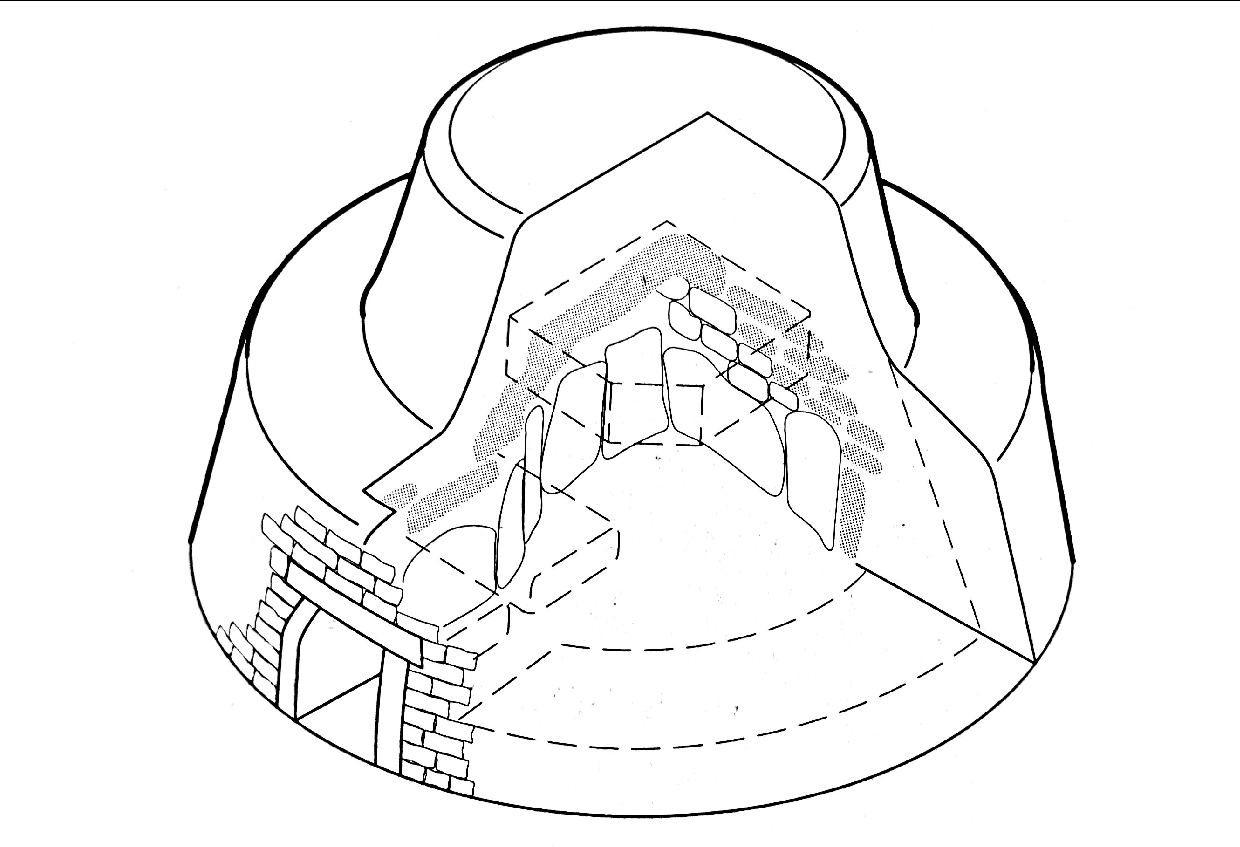
\includegraphics[height=0.4\linewidth ]{figure/Introduction/oldMasonry2.pdf}
\caption{Megalith tomb, Er-Mané,Carnac,Brittany,France,ca 4200 BCE\cite{ref:WorldHistory}}
\end{figure}

Later, about 3000 BCE in Mesopotamia, the first fired bricks appeared, which was a development from the sun dried mud brick used even earlier.
Egypt also built it cities with using of mud bricks, but they unlike Mesopotamia or the Indus valley, had excellent deposits of stone exposed above ground; limestone, sandstone, and granite were all available.
Therefore a new technology of cut-stone construction emerged in the temples and pyramids of the 4th dynasty (c. 2575–c. 2465 bce)\cite{ref:buildConstrBrit}. 

\begin{figure}[H]
\centering
\includegraphics[width=0.9\linewidth ]{figure/Introduction/EgyptArchitecture.jpg}
\caption{Relief depicting god Amun with great helmet covered with two large feathers and beard sitting on the throne. First court of Ramses II. New Empire. Temple of Luxor. Egypt.,Prisma / Universal Images Group
}
\end{figure}

The Romans inherited and refined those building technologies used in earlier civilisations. Even though Romans did master stone masonry it was the brick that would be the most used material. This is due to the big industry that had been emerged and that it became a much more cheap material. Mortar had been used previously in the sense of sand, lime, and water. The Romans introduced a new component in the beginning of the 2nd Century which we now call pozzolana. The combination of lime and pozzolana made the mortar into a natural cement. This made it much stronger and weather resistant and it would prove to even harden under water. Pozzonlanic mortars became a very popular and cheap material and when mixing it with stones it got those properties of concrete\cite{ref:buildConstrBrit}. The most famous example of concrete structures is Pantheon in Rome, which is a dome made of concrete blocks.
\begin{figure}[H]
\centering
\includegraphics[width=0.9\linewidth ]{figure/Introduction/PantheonInt.jpg}
\caption{Pantheon, Neil Emmerson / Robert Harding World Imagery / Universal Images Group
Rights Managed / For Education Use Only, Wikipedia}
\end{figure}


\subsubsection{Historic Forms of Masonry Shells} \label{sec:masonryShells}

The shape of the shell can as Heinz Izler proved take many different shapes. In history of masonry the selection of shells have been restrained to a few. These usually based on rotational surfaces cut by planes or by other rotational surfaces.They can also be combinations of two types of vaults. In the figure below it is possible to see some of the most common from a Swedish book \cite{ref:murning}. Translations are based on a dictionary for architecture \cite{ref:lexi}.


\begin{figure}[H]
\centering
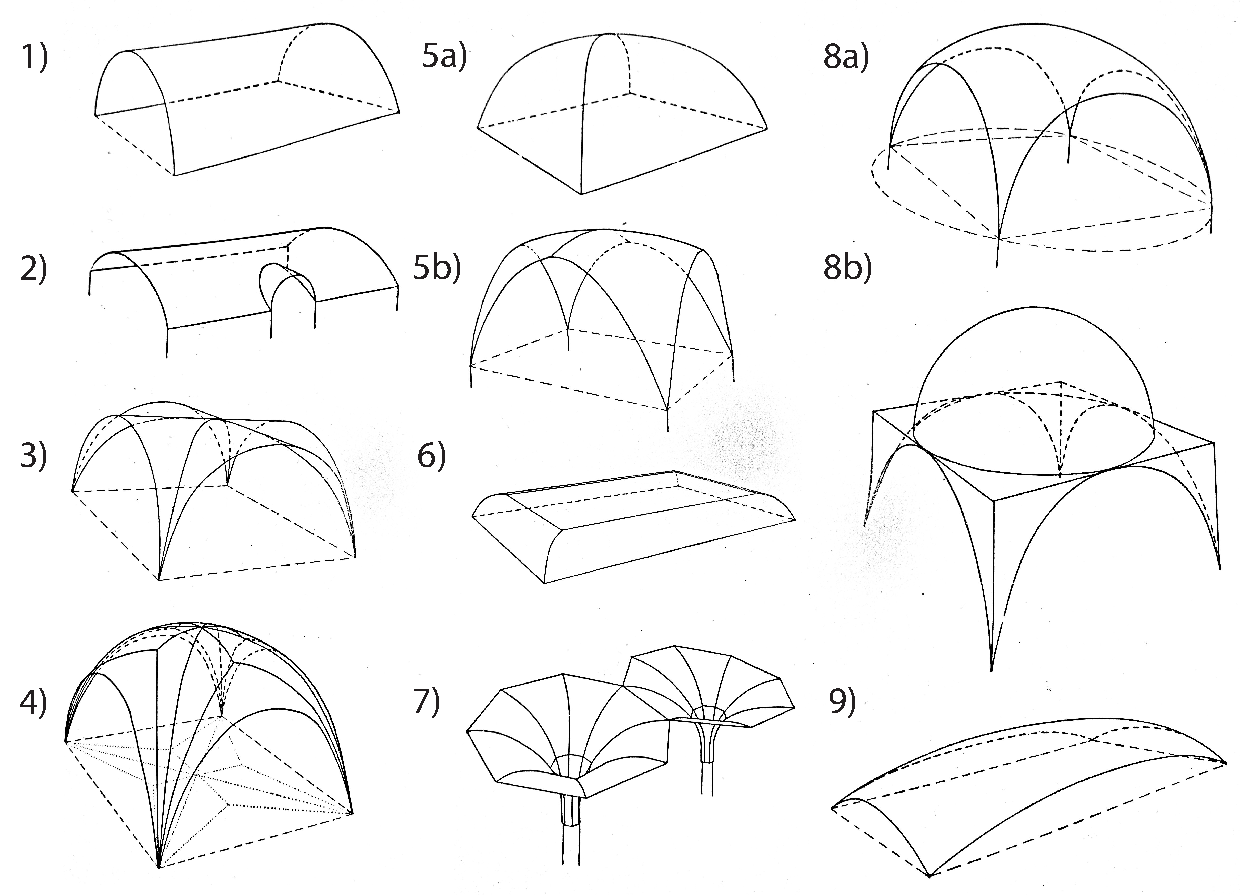
\includegraphics[width=0.8\linewidth ]{figure/Introduction/TypValvNum.pdf}
\caption{Different types of traditional masonry vaults. The a) and b) indicates different variations of the same type´\cite{ref:murning}}
\end{figure}



\begin{enumerate}
    \item \textit{Barrel vault} - The geometry is based on cylinder cut in two half-ways,i.e the two shapes are of the same size after cutting.
    \item \textit{Segmental vault} -  It is similar to a barrel vault, but the cylinder is cut above or below the center-line.
    \item \textit{Groin vault} -  The geometry is achieved when two half cylinder shapes with same diameter and standing on the same plane, but with an 90 degree angle, cuts each other. 
    \item \textit{Stellar vault} - It is based on a form of subdivison of the groin vault.
    \item \textit{Cloister vault} - Constructed geometrically in a similar fashion as the groin vault. Though the cylinder pieces that are above the cutting lines are taken away.
    \item \textit{Cavetto vault} -  This is a combination of Cloister vault and a segmental vault.
    \item \textit{Fan - vault} - The geometry is based on a curve that is rotating around a center line creating a rotational surface.
    \item \textit{Sail vault} - The geometry is based on half sphere which is cut vertically along an inscribed square.
    \item \textit{Saucer dome} - A type of Sail vault but with milder curvature.
\end{enumerate}



\subsubsection{Modern Masonry Shells in Architecture}



The structures of vaults and domes has a strong position in most historic description of Architecture. Two names that stand out in modern time architecture in this genre are \textit{Rafael Guastavino} and \textit{Eladio Dieste}. They are seen as the main contributors to revolutionise the structural arts of masonry shells and take it into the modern era. 
"Until late in the nineteenth century, masonry vaulting was shaped and proportioned by guesswork or rules of thumb. As a consequence, vaults based on the European or Middle Eastern precedents tended to be not only thick but also heavy and expensive. Catalan vaults were much thinner but were also designed by wholly intuitive methods."
Instead of rely on intuition Guastavino used \textit{graphic statics} which was a relatively new method at the time to describe and understand force patterns of structures. Graphic statics made it possible to visualise the optimal shape of vaults and trusses. This in combination with the technique of catalan vaults made it possible to construct very slender structures. "Although Guastavino patented techniques for both reinforcing and post-tensioning, most of his roofs were constructed of unreinforced masonry"





 John Oschendorf describs the legacy of the Guastavino Company \textit{"With complex three dimensional vaults, supported by carefully placed stiffening walls, flying buttresses, and tension ties, the Guastavinos worked as master masons in the modern era"} 

\begin{figure}[H]
\centering
\includegraphics[height=0.4\linewidth ]{figure/Introduction/GuastovinoStair.jpg}
\includegraphics[height=0.4\linewidth ]{figure/Introduction/GuastavinoStair2.jpg}
\caption{Tile vaulted staircase of Baker Hall, Carnegie Mellon University, Pittsburgh, 1914. Courtesy of Michael Freeman.}
\end{figure}

Dieste did in comparison to Guastavino use formwork during construction and worked only with steel reinforced and often post tensioned structures.Instead of using Graphic Statics Dieste used numerical methods to design his structures. "Dieste’s building structures fall into four general categories, none of which was feasible in Guastavino’s time."

\begin{itemize}

\item Gaussian Vaults
\item Self supporting shells
\item Folded structures
\item Ruled surfaces
\end{itemize}

\begin{figure}[H]
\centering
\includegraphics[width=0.4\linewidth ]{figure/Introduction/DiesteFour.JPG}
\caption{The four categories of Dieste Eladio Dieste: innovation in structural art}
\end{figure}

"There were others as well who built with reinforced brickwork, but two things set Dieste’s work above the rest. One is his unmatched use of masonry in structures subject to bending, such as cantilevered barrel shells, tanks under hydrostatic pressure, and folded plates. The other is the power and poetry of his masonry architecture."


Important contemporary initiatives to develop the art and understanding masonry shells is the Block Research Group at ETH in Zuring which is directed by professor Philippe Block and Dr. Tom Van Mele. BRG has since the start specialized in the field of computational methods applied to masonry and concrete shells. Their research have enabled new forms of equilibrium masonry shells that previously was not possible previously. Below is a project that was built on the ETH campus by BRG where the free form shape was designed and validated using Thrust Network Analysis,which was developed by Block under the guidance of John Oschendorf at MIT. \cite{ref:Davis} To read more about TNA read section \ref{sec:TNA}. 

\begin{figure}[H]
\centering
\includegraphics[width=0.9\linewidth ]{figure/Introduction/Block_Vault.jpg}
\caption{Surface and contour plots showing $z(x,y)=\sin(x+y)\cos(2x)$.}
\end{figure}

\subsection{Shell Structures}

Vaults, cones and domes are the forms that are typically associated as shell structures. In architecture it is common for shell structures to consist of concrete bricks and stone. In modern times it can be reinforced using steel but historically it has been unreinforced. A shell could also be a car or plane body or a birds' eggs. Williams \\

Mentioning the most obvious shell form there are many different shapes of the shell, described by Heinz Isler.

\begin{figure}[H]
\centering
\includegraphics[width=0.6\linewidth ]{figure/Introduction/ShellDiagram.jpg}
\caption{Shell diagram over different types of shell by Heinz Isler}
\end{figure}

As Williams state there are many ways to describe a shell, but the most obvious definition might be through its geometry.

"A shell is a structure defined by a curved surface it is thin in the direction perpendicular to the surface, but there is no absolute rule as to how thin it has to be. It might be curved in two directions, like a dome or a cooling tower, or it may be cylindrical and only curve in one direction." Williams Architecture Shell.

In the book Shell Structure you can read this definition of a shell structure taking its.

"Shell Structures are constructed systems described by three-dimensional curved surfaces, in which one dimension is significantly smaller compared to the other two. They are form-passive and resist external loads predominately through membrane stresses." Introduction 

A form-passive structure meaning that you do not experience much degrees of change of shape or form. Where a form-passive would break under high deflection a form-active can adapt to a new equilibrium state like cables or membrane structures. Source needed? 
Membrane stress and membrane structures should not be mixed up. Membrane condition is when the forces are mainly carried in the plane of the shell surface. Membrane stresses can be in compression, tension or a combination of them both. \\



In the book Shell structures for Architecture optimisation it distinguish between three types of geometries for Shell Structures, and defined as following.




\begin{itemize}
\item Freeform, free-curved or sculptural shells are generated without taking into consideration structural performance.  
\item Mathematical, geometrical or analytical shells are directly described by analytical functions.These functions are of then chosen for their convenience in performing further analytical calculations and their ability to describe a shell's shape for fabrication purposes.
\item Form Found shells include natural, hanging shapes assosiated with funicular structures of Antoni Gaudi, Frei Otto and Heinz Isler, but also "strained" gridshells tat feautre bending stresses. Their final shape is a result of attaining a state of static equilibrium.
\end{itemize}



\subsubsection{Gridshells}


"A gridshell is essentially a  shell with its structure concentrated into individual members in a relatively fine grid compared to the overall dimensions of the structure. The members may be short and only pass from node to node, or they may be continuous, crossing each other at the nodes. The grid may have more than one layer, but overall thickness of the shell is small compared to the overall span" p89

Common materials for gridshells have been timber and steel. Examples of timber gridshells are Mannheim Multihalle, by Frei Otto, Downland Gridshell and 

\begin{figure}[H]
\centering
\includegraphics[width=0.3\linewidth ]{figure/Introduction/DownlandC.jpg}
\includegraphics[width=0.3\linewidth ]{figure/Introduction/Downland.jpg}
\includegraphics[width=0.3\linewidth ]{figure/Introduction/Savill.jpg}
\caption{Multihalle and Downland Gridshell}
\end{figure}

\begin{figure}[H]
\centering
\includegraphics[width=0.9\linewidth ]{figure/Introduction/TheGreatCourt.jpg}
\caption{British Museum court roof}
\end{figure}




\subsection{Geometrical Challenges}



It is very tempting to try as a designer to map patterns made on paper onto a 3d shape. Take the finished drawing and drape it onto the surface. That would for many reasons be very effective. The most prominent one is that one could build 3d dimensional surfaces or objects with single element and it would give a big free-dome to the designer. The problem is that it merely impossible, unless you have say a cylinder, you can always role a paper into a cylinder, it is just not that fascinating. 

\begin{figure}[H]
\centering
\includegraphics[width=0.8\linewidth ]{figure/Introduction/drape.jpg}
\caption{}
\end{figure}

This is not a problem only concerning architects and engineers. Since we started travelling and using maps as guides this has somewhat been a problem, how do you make something that has the shape of a sphere two dimensional?A solution to this problem was discovered by  \textit{Gerardus Mercator} in 1569, a so called \textit{Mercator Projection}\cite{ref:merc}. This is basically a method to project a sphere onto a cylinder that can be unrolled to a plane. This is of course not true since the projection becomes different depending on your distance to the equator, and the poles can not even be projected. 550 years later this method is still used in applications such as \textit{Google Maps}\cite{ref:maps}. This proves that even for such simple shape as the sphere it is really hard finding a mathematical solution. Going back to architecture there is a big difference and that is that the geometry does not have to be sphere, it just need to look like it. A brick corner is never perfectly straight due to irregularities in the stone or mortar, but we observe it as straight. This gives a bit more free-dome to tweak the mathematics and allow some deviance from the mathematical shape to suit the kind of structural representation of choice. Mercator still present today proves though that we always should enter the field of geometry mapping with soft and humble eyes. Sometimes reality is hard, and that is ok.

\begin{figure}[H]
\centering
\includegraphics[width=0.9\linewidth ]{figure/Introduction/Mercator.jpg}
\caption{The length of the curve is the same regardless of coordinate system.Cylindrical Projection on the Earth. [Illustration]. Encyclopædia Britannica ImageQuest}
\end{figure}



\subsubsection{Stereotomy }
  
Stereotomy is defined as "the science or art of cutting solids into certain figures or sections". It includes, and the term is sometimes used as a synonymous with, the art of cutting stones for masonry shells. From Notes of Stereotomy.

\begin{figure}[H]
\centering
\includegraphics[width=0.45\linewidth ]{figure/Introduction/NotesonStereotomy.JPG}
\includegraphics[width=0.45\linewidth ]{figure/Introduction/NotesonStereotomy2.JPG}
\caption{The length of the curve is the same regardless of coordinate system.}
\end{figure}

It was used early as an tool for subdividing shapes into building elements that would be able to cut and fit together. Wellknown in this field is Philibert de l'Orme from France that was active during the 16 th century. Long before computers practitioners of stereotomy managed to create astonishing structures and patterns of very complex surfaces.

\begin{figure}[H]
\centering
\includegraphics[width=0.90\linewidth ]{figure/Introduction/Arles.jpg}
\caption{The length of the curve is the same regardless of coordinate system.}
\end{figure}

This techniques are not very common today since it involves quite complex building elements that need to be manufactured. Though it is possible to read the research of the Block research group where they have investigated in how to use computational methods and digital fabrication to achieve this structures.

\begin{figure}[H]
\centering
\includegraphics[height=0.50\linewidth ]{figure/Introduction/StereoBlock2.JPG}
\includegraphics[height=0.35\linewidth ]{figure/Introduction/StereoBlock.JPG}
\caption{The length of the curve is the same regardless of coordinate system.}
\end{figure}



\begin{figure}[H]
\centering
\includegraphics[height=0.4\linewidth ]{figure/Introduction/blockStereo.jpg}
\caption{The length of the curve is the same regardless of coordinate system.}
\end{figure}


\subsubsection{Brick patterns on shell structures} \label{sec:brickPatt}

It is a rather delicate geometrical problem how to cover a surface or a shell with bricks. It is quite  different to, for instance stereotomy,  since the brick format, a cuboid, is a fixed constraint and in stereotomy the elements almost obeys the form and you can have many different element types. The advantage of brick structures  is that the bricks has a flexible connection which means that the perpend joints does not need perfectly equal. This gives a certain amount of freedom for the architect, engineer o brick layer to allow certain voids and irregularities which would have been disastrous for other types structural systems. One can see the brick structures as discrete version of the surface, like quadrilateral mesh, since the bricks, for at least curved objects, never will be in-line with the surface. 
\begin{figure}[H]
\centering
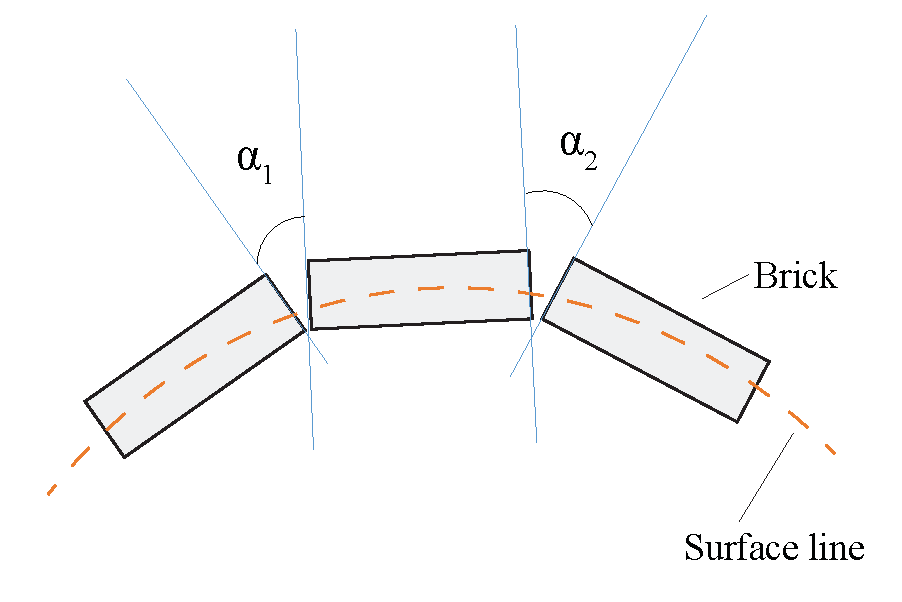
\includegraphics[width=0.8\linewidth ]{figure/Introduction/brickgeo2.pdf}
\caption{The three main types vaulting}
\end{figure}

The important thing is that the deviations from the form  is firstly, within margins for what can be considered safe from structural point of view, and secondly and what the human eye can observe as smooth surface.The first point is obviously the most important but the second could tested.  

\begin{figure}[H]
\centering
\includegraphics[width=1.0\linewidth ]{figure/Introduction/meshdistort2.JPG}
\caption{The three main types vaulting}
\end{figure}



There has not been much research in finding methods of estimating the brick patterns on complex shapes and surfaces. During a presentation at Harvard with John Ochsendorf from 2011 \cite{ref:interview}, who is a professor at MIT specialised in building technology of masonry structures, gets a question if there are computational methods for generation of brick tilings. According to Ochsendorf there have been attempts to make computational methods that generates brick patterns but without much success, and that he rather believed in experience and intuition of the craftsmen to understand the limits and possibilities for different tiling. He highlights the skills and knowledge that has been lost in this field compared to what The Guastavino Company managed to construct in the beginning of the 20th century.Rather using traditional vaulting as the finishing layer the visible patterns were tiled from beneath. \textit{Following the success of the City hall Station(1904) and St Paul's Chapel in New York in the early 1900s, the Fuastavino company built increasingly sophisticated decorative patterns in its vaulting. This was accomplished by adding the exposed layer of tile last. In other words, masons constructured the vaulting with a rough interior finish, and then applied a final decorative  layer of tile from below.}\cite{ref:Ochsendorf}. This is





\subsection{Brick patterns on traditional vaults}

Reading old masonry handbooks \cite{ref:murning} one can find patterns for traditional vault or shell forms , as described in section \ref{sec:masonryShells}. It is though hard to find records on these have been generated or estimated, and sometimes there are different alternatives patterns for the same form. 

\begin{figure}[H]
\centering
\includegraphics[height=0.8\linewidth ]{figure/Introduction/vaultin2.pdf}
\caption{The three main types vaulting}
\end{figure}


\begin{figure}[H]
\centering
\includegraphics[height=0.60\linewidth ]{figure/Introduction/vaulting1.pdf}
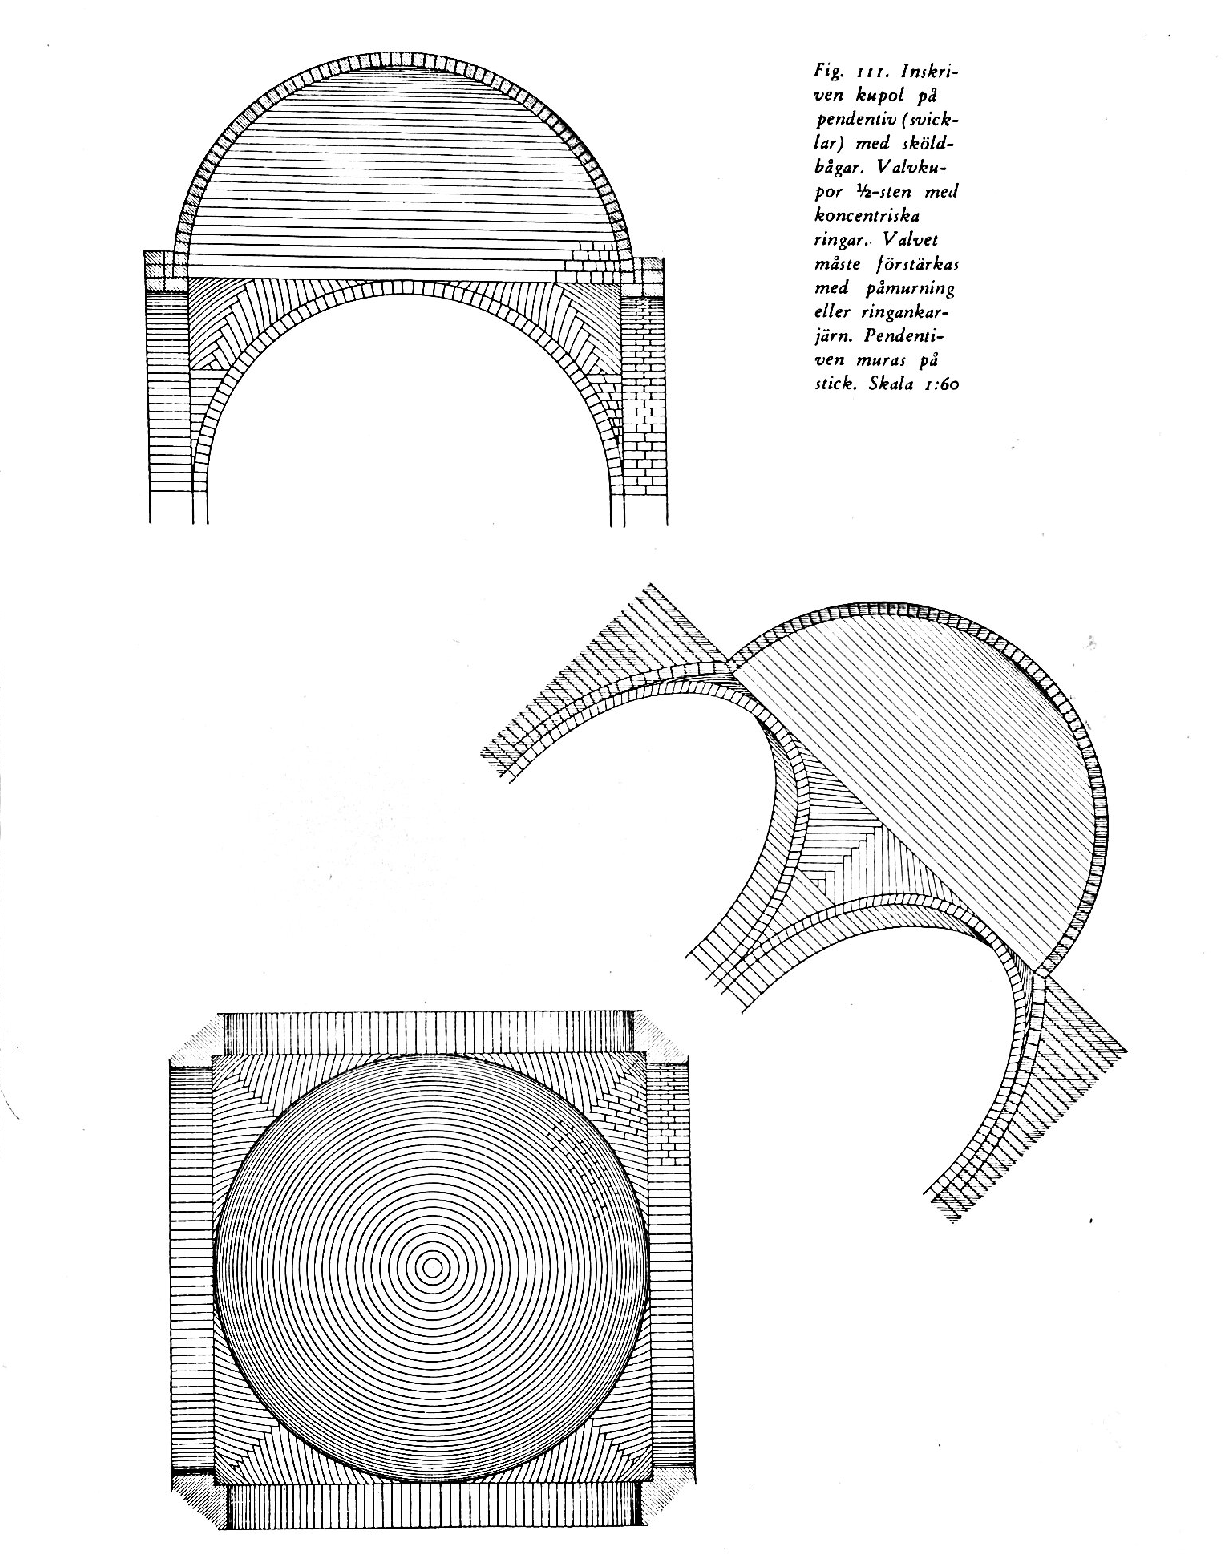
\includegraphics[height=0.60\linewidth ]{figure/Introduction/vaulting3.pdf}
\caption{The three main types vaulting}
\end{figure}

  

\subsection{Brick Structures}

What is typical for a brick structure is uniformity of its building elements, the brick. The brick is made of clay can be formed into nearly any shape, but the most common format is the cuboid. The way the brick is made affects its colour, shape, texture, strength, Resistance to fire and weather and longevity. This means that strangely enough both the diversity and the unity are the most striking features of the structure. Looking at a traditional building the brick composition becomes a patchwork of different colours, the shape has small deviations due to imperfections of the shape and the roughness of the texture. Even though we have modern techniques and methods to make the colours, shape and texture uniform it is mostly common to keep or resemble these imperfections.\\
Two other important aspects of a brick structure is the mortar and the skills and creativity of the craftsman. The mortars main purpose is to bond the bricks together into a structure and to evenly distribute the stress and compensate the differences of the bricks. 

\begin{figure}[H]
\centering
\includegraphics[width=1.0\linewidth ]{figure/Introduction/Rohsska.jpg}
\caption{Rhösska museum in Gothenburg.}
\end{figure}





\subsubsection{The brick}
 
 What defines the brick is  usually the format and the material.  A good definition is made by Mitchell, \textit{Bricks are an artificial kind of stone, made of burnt or baked argillaceous or clayey earth, and the quality  depends upon (a) the chemical properties of the earth, (b) the preparation of the earth, and (c) the different degrees of burning and baking} \cite{ref:Mitchell}.
 There are many different types of clays, or silicate of alumina, with different chemical compositions. Mitchell gives a thumb-rule for a good clay, or brick earth, \textit{"Silica, three-fiths; alumina, one fifth; iron, lime, magnesia,manganese, soda and potash forming the remaining fifth"}\cite{ref:Mitchell}. To get a more detailed view of chemical composition for different clays, see table below. 


\begin{table}[H]
    \centering
    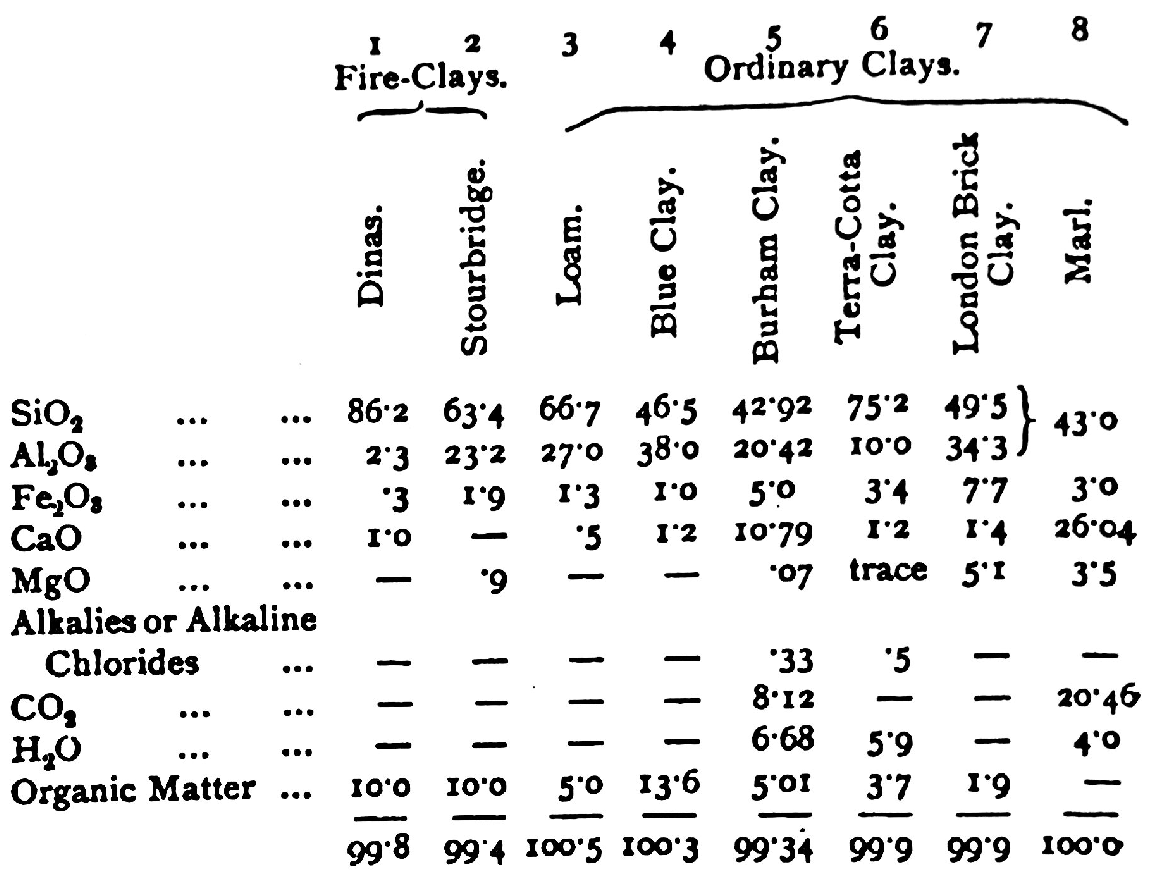
\includegraphics[width=0.7\linewidth ]{figure/Introduction/clays.pdf}
    \caption{ A table that shows the chemical composition types of .  Remake of table in   \cite{ref:Mitchell}}
    \label{tab:my_label}
\end{table}

\subsubsection{Brick formats and terminology}

A fundamental property of the brick wall is as mentioned the unity of the single format. There are though many different types of formats and it is usually a historical or cultural tradition that defines the dimensions in each country. The most common Swedish brick format is for instance a bit larger than the Danish brick dimension. Usually the bed joint height is set depending on the brick to give an even number at say the 5th and 10th layer.The figure belows shows some different brick sizes and the associated height of the bed joint.

\begin{figure}[H]
\centering
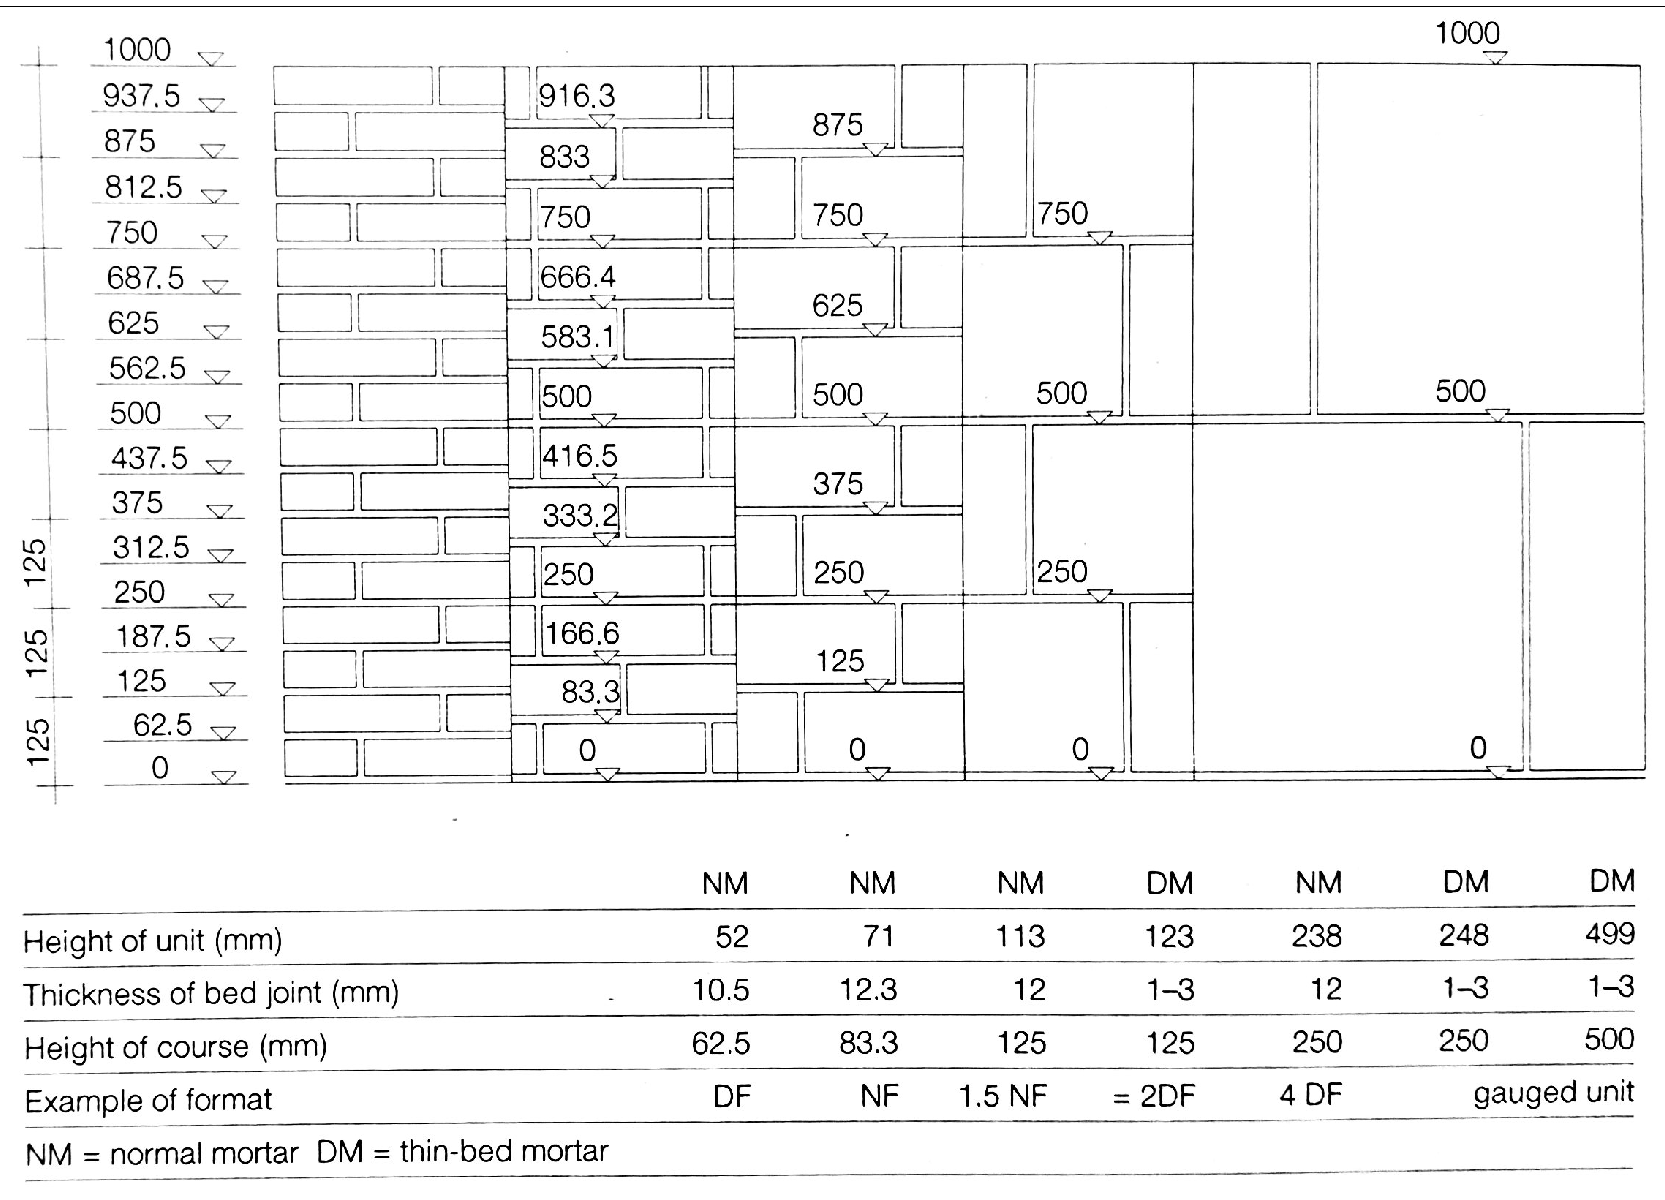
\includegraphics[width=0.9\linewidth ]{figure/Introduction/brickmeasures.pdf}
\caption{\cite{ref:Pfeifer}}
\end{figure}

The brick composition has common terminology and the name of the brick sides are determined by which edge is facing the bed joint. The most common placement is the stretcher and header, see figure below. The bed joint is the the mortar joint between the courses, one layer of bricks are called a course, and the the vertical joint is called perpend. Bats are is a piece of a brick, 1/2 or 3/4. The bats can be fabricated but the brick layer must also be able make them himself by splitting the brick the right size with his hammer.\cite{ref:Mitchell}

\begin{figure}[H]
\centering
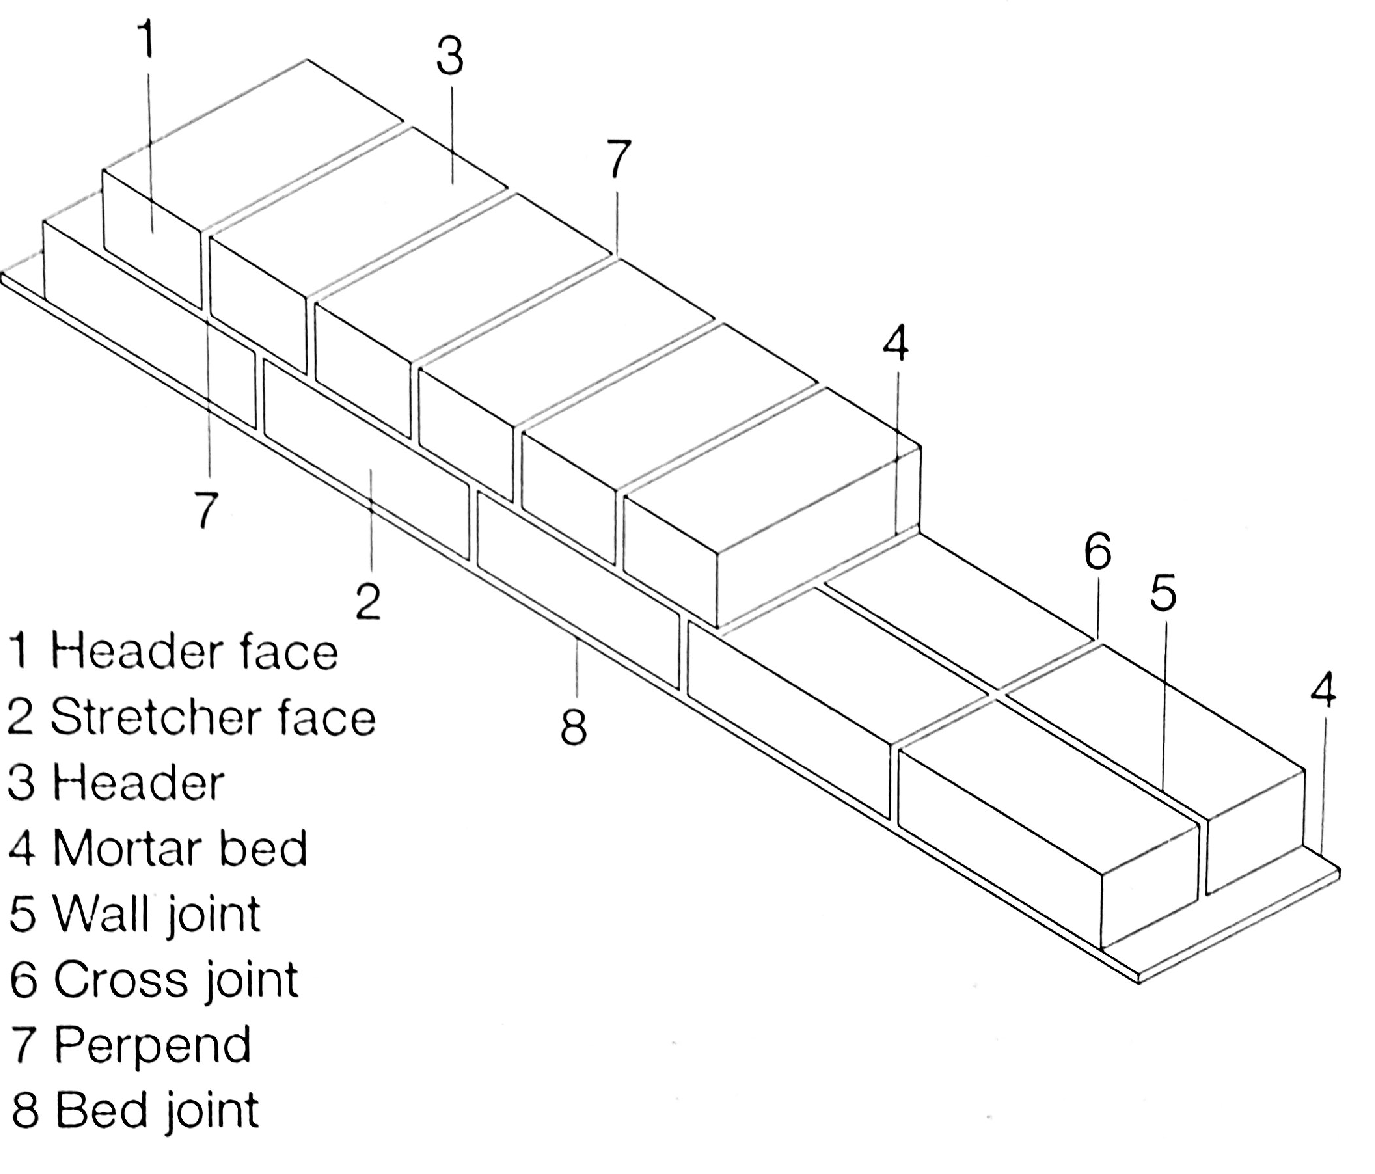
\includegraphics[width=0.6\linewidth ]{figure/Introduction/brickterm.pdf}
\caption{\cite{ref:Pfeifer}}
\end{figure}




\subsubsection{Material Properties}

Bricks belongs to the group of materials called ceramics. Bricks are made
There are some general properties that applies to clay based ceramic materials.\\

\begin{itemize}
\item Hard and brittle
\item Momentanelastiska(engelska??),
i.e. they have almost no creep and plastic deformation
\item Thermal resistant(värme beständinga)
\item Resistant against acid and biological attacks
\item Have small volumetric deformations,
i.e. no deformations related to heat and moisture.
\item High electrical resistivity  (elektriskt isolerande)
\end{itemize}

The mechanical of physical properties of bricks are that they are very favourable under pure compression. The very high compressive strength is in contradiction to it tensile and flexural capacity. 

\begin{figure}[H]
\centering
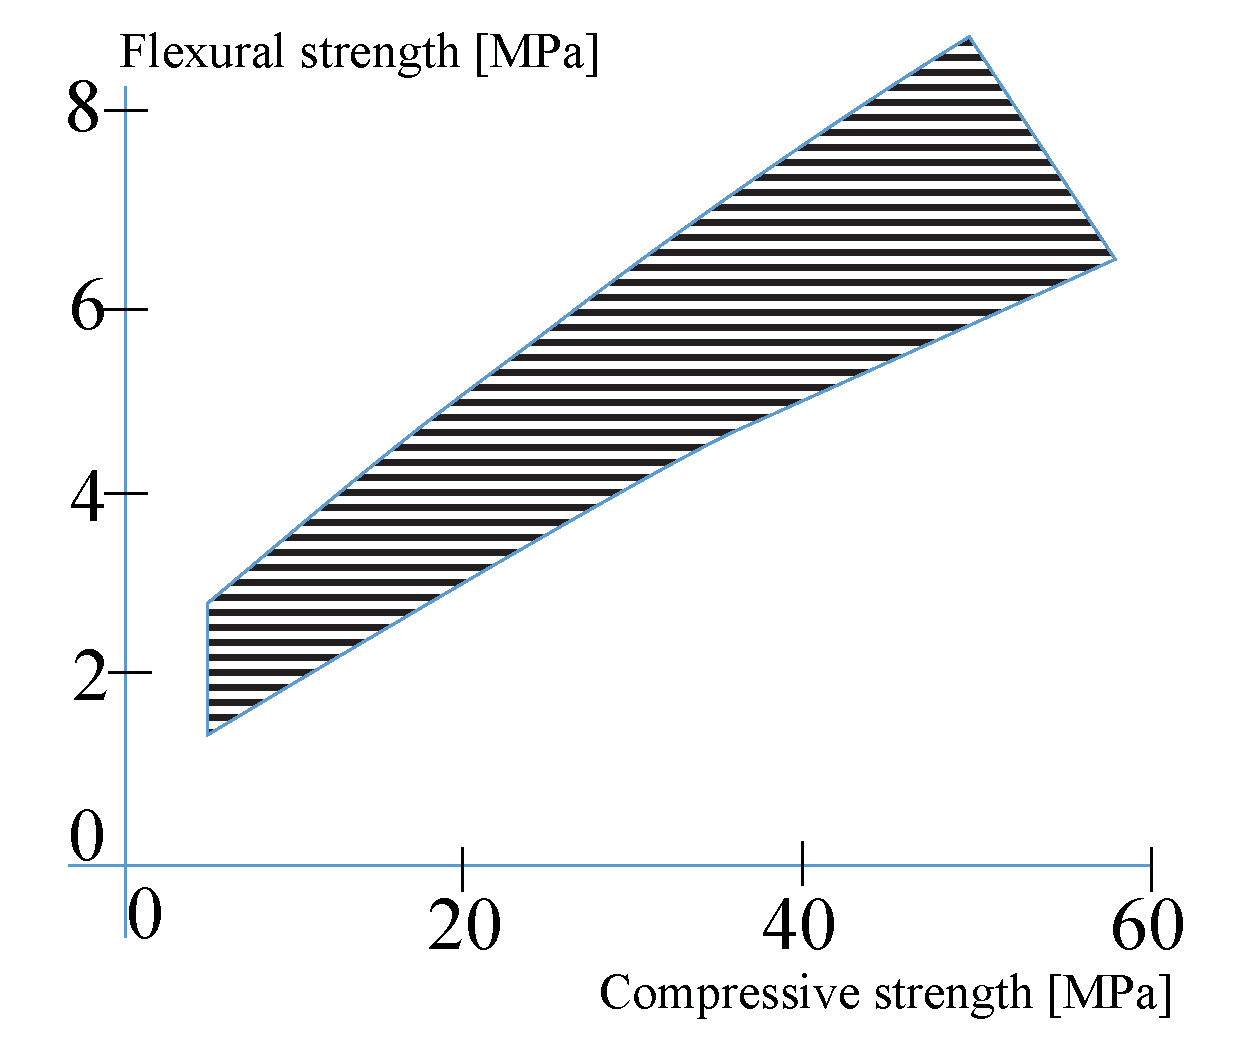
\includegraphics[width=0.49\linewidth ]{figure/Introduction/BrickProp1.pdf}
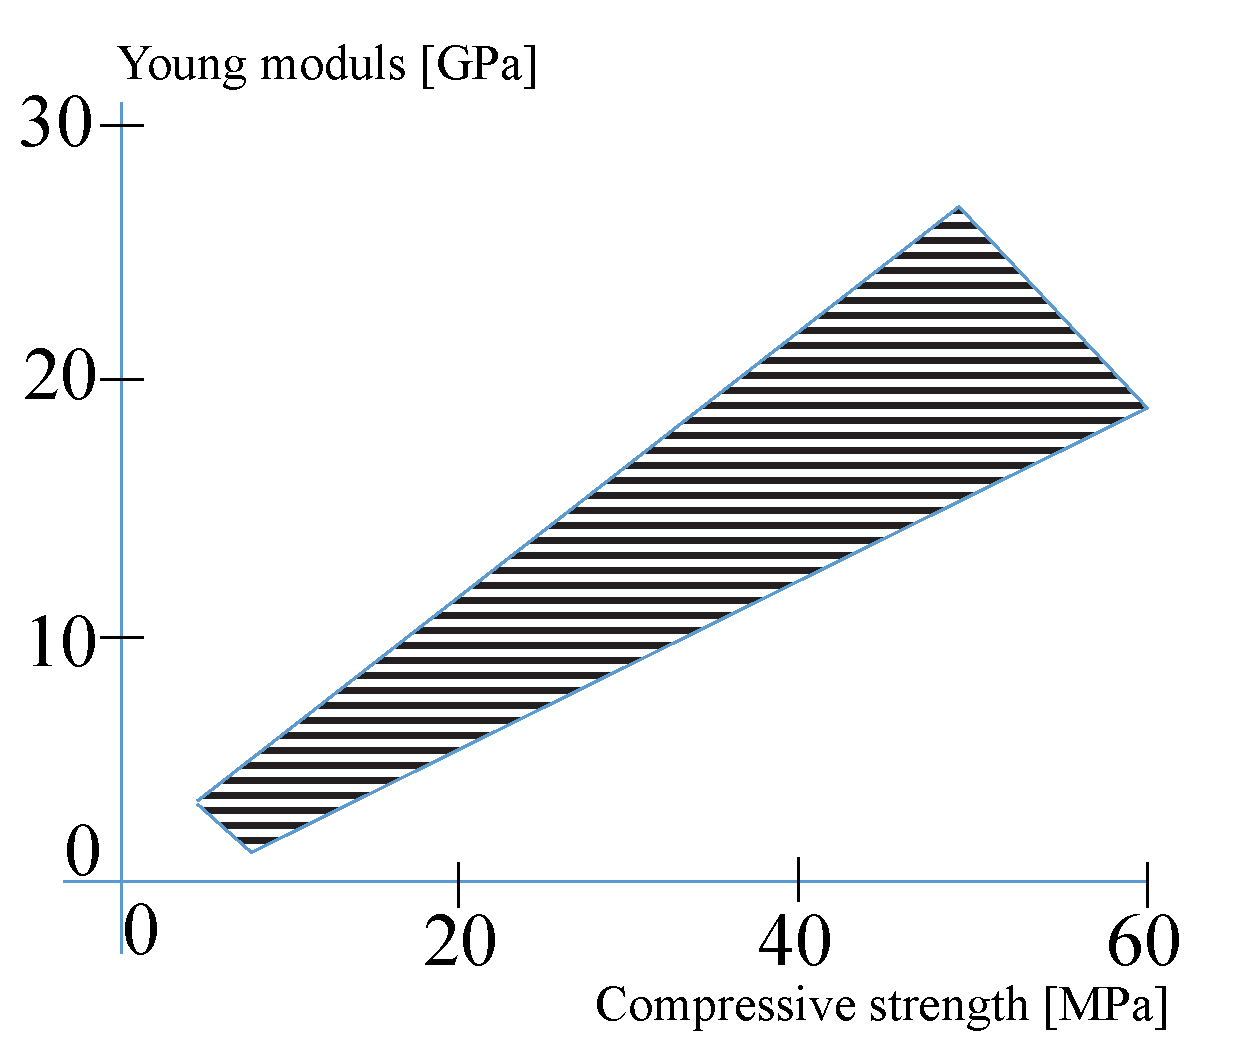
\includegraphics[width=0.49\linewidth ]{figure/Introduction/BrickProp2.pdf}
\caption{Two graphs that shows the mechanical properties of bricks. These pictures are remakes from\cite{ref:byggmaterial} }
\end{figure}

Notice the very low Elasticity modulus compared to for instance steel which could go well over 200 GPa, the table below shows the elasticity modulus of various materials.
\begin{figure}[H]
\centering
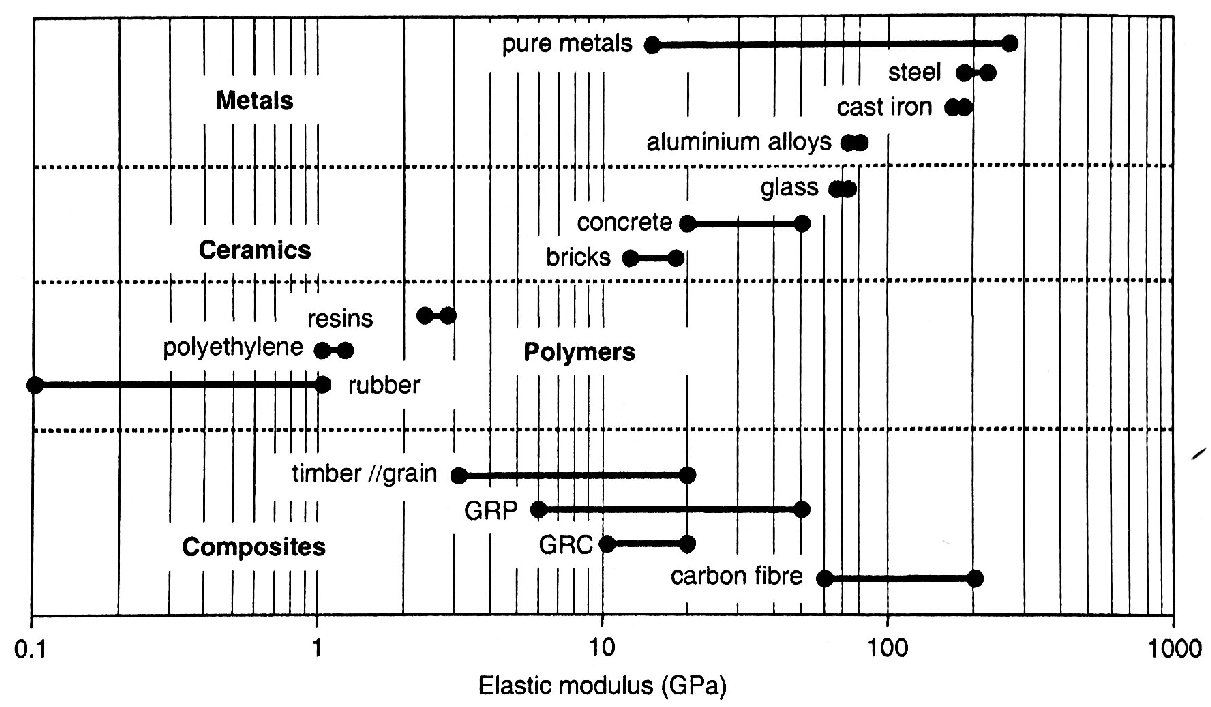
\includegraphics[width=0.9\linewidth ]{figure/Introduction/elastictymodulus.pdf}
\caption{A graph from a Swedish text book \cite{ref:byggmaterial} that shows how various properties is affected by the kiln temperature}
\end{figure}



The exact properties are much related to the composition of the raw material and the kiln temperature. The graph below shows how for instance the density and the pore properties change with the temperature.

\begin{figure}[H]
\centering
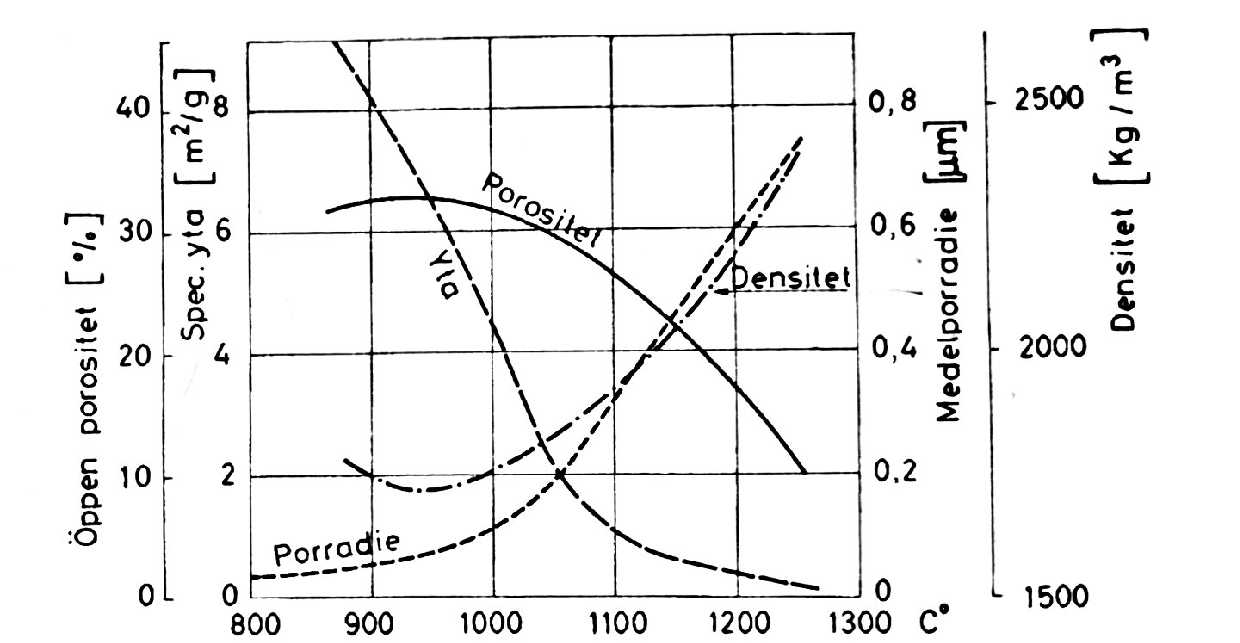
\includegraphics[width=0.9\linewidth ]{figure/Introduction/brickProp3.pdf}
\caption{A graph from a Swedish text book \cite{ref:byggmaterial} that shows how various properties is affected by the kiln temperature}
\label{fig:brickProp}
\end{figure}



\subsubsection{Brick Making}

The fabrication of the brick is very crucial for the performance of the brick structure. Many of the properties are closely related to composition of the brick earth \cite{ref:Mitchell} and the kiln temperature, see figure \ref{fig:brickProp}.
The brick fabrication can be divided into the following steps.\cite{ref:byggmaterial} 

\begin{enumerate}
    \item Preparation of the raw material
    \item Forming of the bricks
    \item Drying
    \item Burning and cooling
    \item Sorting
\end{enumerate}

The forming of the bricks is a quite an important step for the format of the brick. There are two main principles.

\begin{enumerate}
    \item the machine made, wire-cut, figure \ref{fig:wire}
    \item The machine-made pressed, or hand moulded, figure \ref{fig:mould}
\end{enumerate}

The wire-cut bricks usually get very precise and smooth surface, the look is quite industrial. The pressed or moulded bricks can get quite rough and the shape is usually a little bowed, curved or twisted. Worth mentioning that this is not a problem due to the adaptability of the mortar joints. 

\begin{figure}[H]
\centering
\includegraphics[width=0.9\linewidth ]{figure/Theory/wireBrick.jpg}
\caption{An industrialised way of making bricks using a wire-cutter\cite{ref:tegel}}
\label{fig:wire}
\end{figure}

\begin{figure}[H]
\centering
\includegraphics[width=0.3\linewidth ]{figure/Theory/brickmaking2a.jpg}
\includegraphics[width=0.3\linewidth ]{figure/Theory/brickmaking1.jpg}
\includegraphics[width=0.3\linewidth ]{figure/Theory/brickmaking2b.jpg}
\caption{A traditional method of brick making is by putting it into wooden forms. Today this is not very common and the bricks are usually pressed by a machine. \cite{ref:tegel}}
\label{fig:mould}
\end{figure}

There are some different kinds of kilns. The principles are though the same even though they can be constructed differently. Below is a figure describing a tunnel kiln and the different stages of the process.




\begin{figure}[H]
\centering
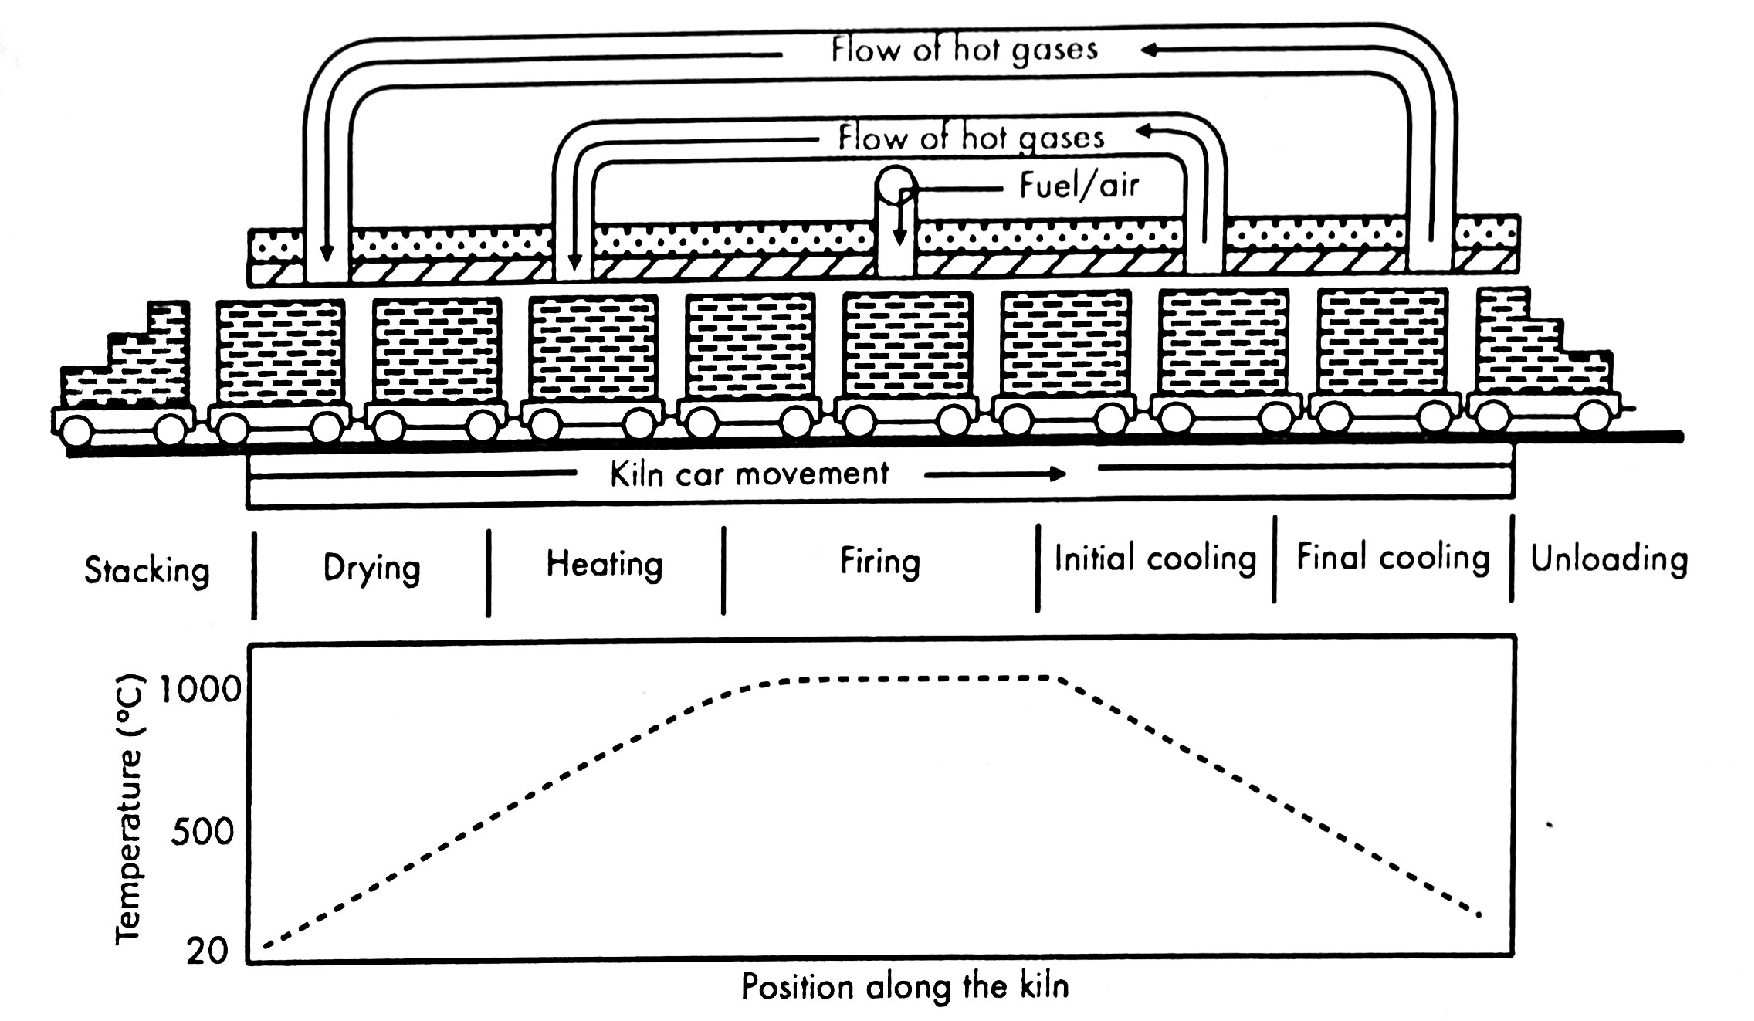
\includegraphics[width=0.9\linewidth ]{figure/Introduction/kiln2.pdf}
\caption{Principles of a tunnel kiln. Above is the different stages and below one can follow the difference in temperature during these stages \cite{ref:ConstructionMaterials}}
\end{figure}


\subsubsection{Mortar}

Mortar is  material used in building construction to bond brick, stone, tile, or concrete blocks into a structure. Mortar consists of inert siliceous (sandy) material mixed with cement and water in such proportions that the resulting substance will be sufficiently plastic to enable ready application with the mason’s trowel and to flow slightly but not collapse under the weight of the masonry units.\cite{ref:mortar}

Main ingredients of mortar are:
\begin{itemize}
\item \textit{Water}
\item \textit{Aggregates} - The aggregates in mortar is mostly \textit{sand}. Sand is a rock mixture of rock particles of different sizes from 10 mm in diameter down to 75$\mu$m. 
\item \textit{Binder} - Widely used binders are based on one of these categories
    \begin{itemize}
    \item \textit{Hydraulic cements}, which reat chemically with water at normal site temperatures.
    \item \textit{lime-silica mixtures}, which react only in the presence of high-pressure steam.
    \item \textit{lime-pozzolan mixtures}, which set slowly at ambient temperatures, or pure lime which sets slowly in air by carbonation.
    \end{itemize}
\item \textit{Admixtures}, examples of are: plasticisers,super plasticisers,accelerators, retarders, air entraining agents. 
\item \textit{Pigments}
\end{itemize}





\subsubsection{Craftsmanship}

The art of bricklaying is to combine  bricks with mortar, which is a workable paste in its initial state that binds the bricks together, to form a composition of structural elements. This composition must meet the requirements of the engineer or architect in terms or geometrical, aesthetic, structural and thermal requirements (it should be dense so that water and air cannot directly pass through). It is a very unforgiving craft since you have no margins for error due to the quick setting of the mortar. If the craftsmanship has been lacking it is very time consuming and require much effort to correct or repair afterwards. 

What differs the brick layer from other crafts is the pure simplicity, not much has changed with time and the execution is still very traditional. A description from Swedish text book for bricklayers states \textit{ For brick laying only a few tools are required: spatula, hammer( specialized for cutting bricks), plump, spirit-level,cord and corner sticks\cite{ref:murning}.}

\begin{figure}[H]
\centering
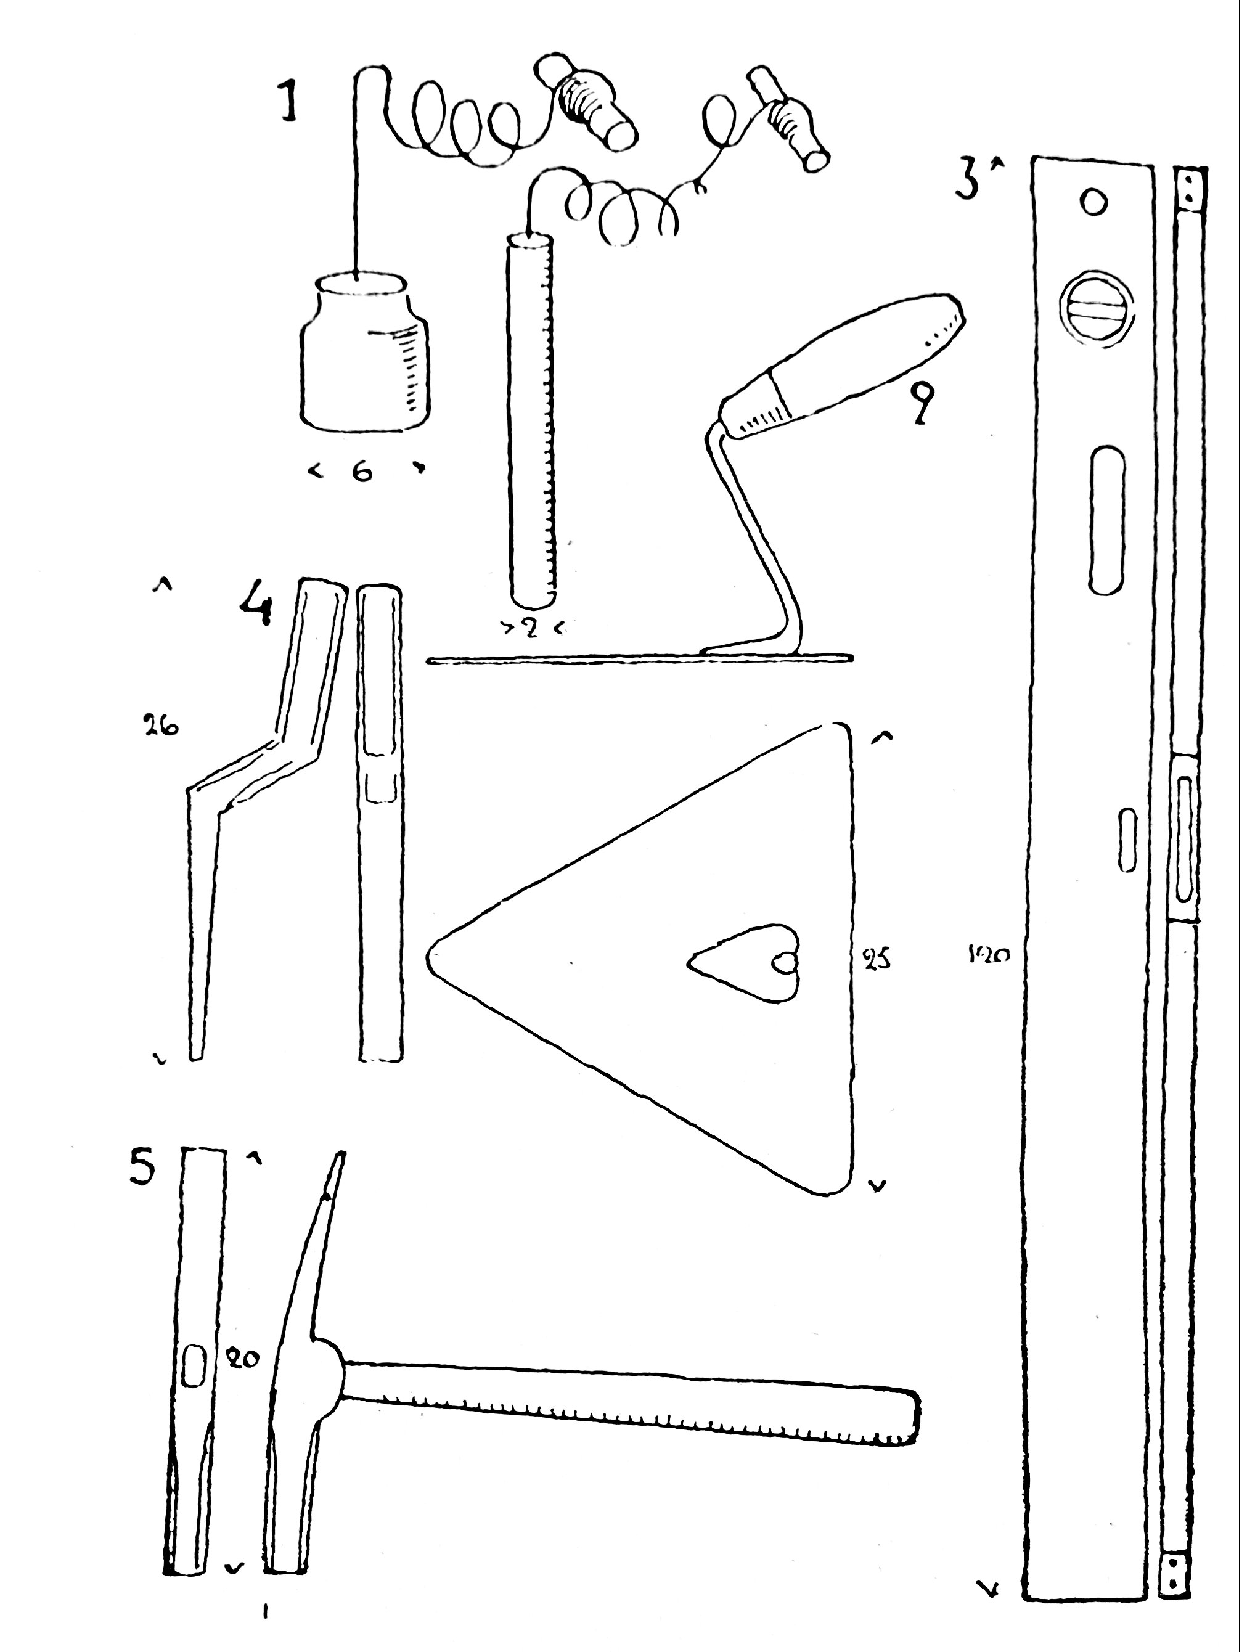
\includegraphics[width=0.4\linewidth ]{figure/Introduction/tools2.pdf}
\caption{Typical tools for a brick layer from a Swedish  brick layer handbook from 1938. 1)Plumb 2)spatula(looks like a 9) 3)spirit level 4)Wooden jointer 5)Hammer for brick cutting  \cite{ref:murning}}
\end{figure}

With the spatula the brick layer applies just enough mortar to make the brick attach to the underlying brick and assures the bed joint height is level.It is also important to apply enough mortar and pressure in the placement of the vertical joint,figure \ref{fig:murning2}  The hammer is used to cut the stones for situations where the normal format does not fit, it can be at corners or vaults.
The most common technique of keeping the brick level is to work with a cord attached between two corners sticks, figure \ref{fig:murning}. This they due whenever possible  to do so. When not possible a brick layer must be able to work with only a spirit level and plump to keep ensure the geometrical entities level,figure \ref{fig:murning2}. The working stages is illustrated in the illustrations below.  

\begin{figure}[H]
\centering
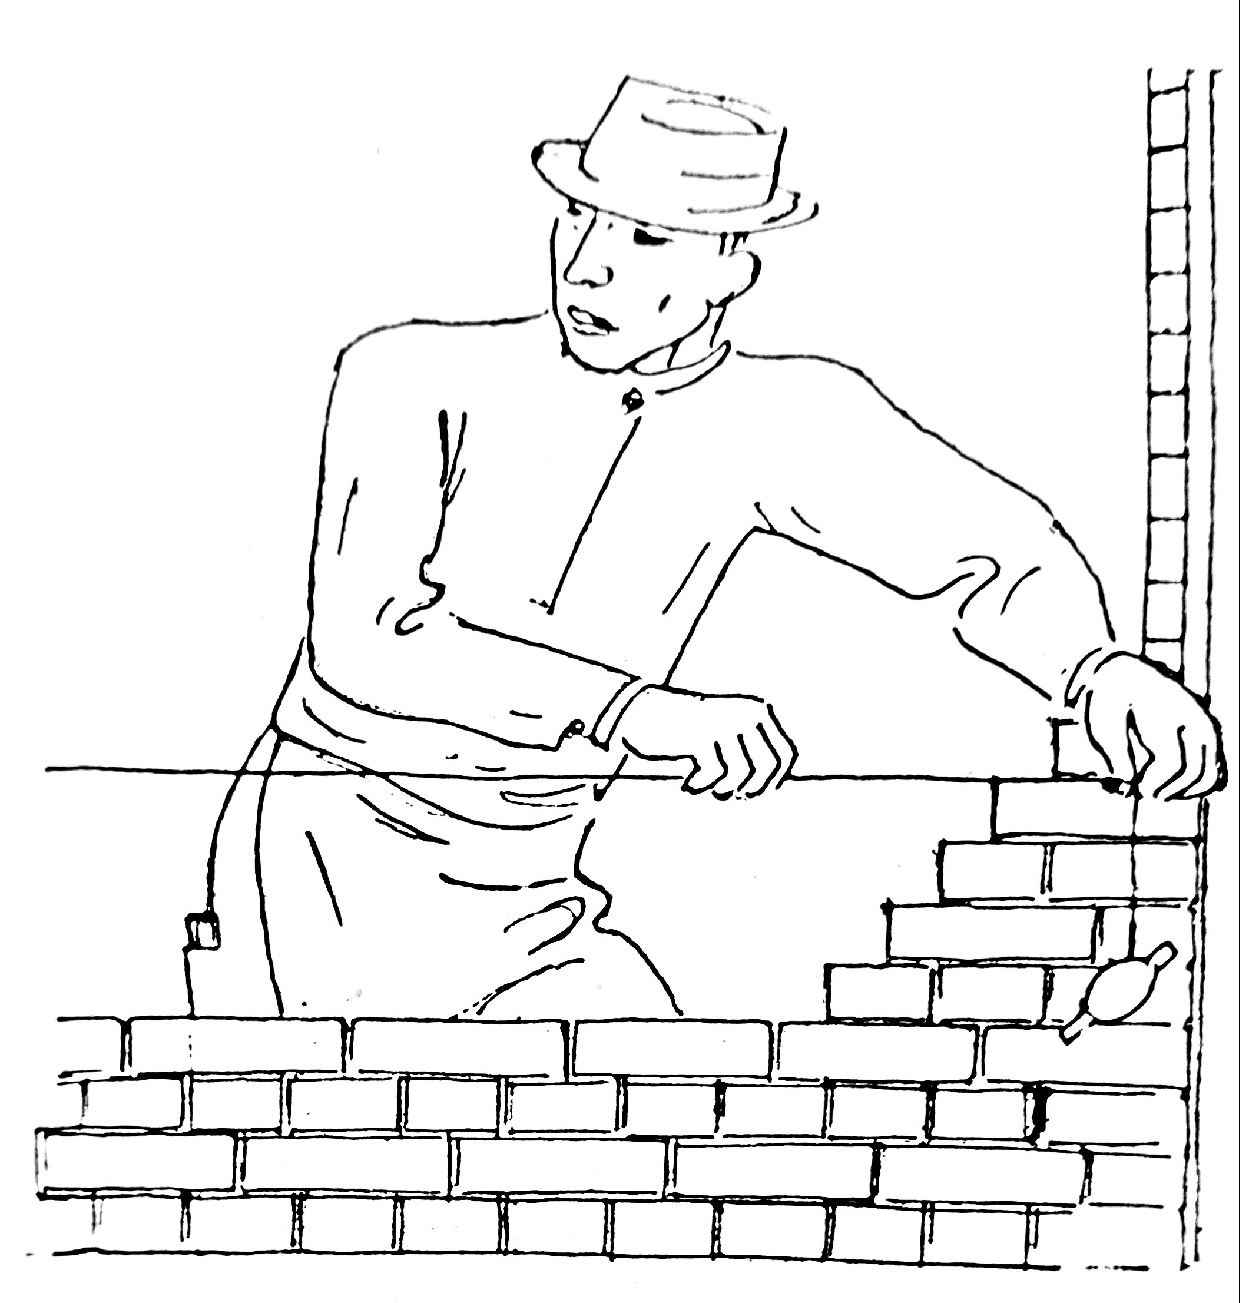
\includegraphics[width=0.40\linewidth ]{figure/Introduction/bricklay4.pdf}
\caption{The length of the curve is the same regardless of coordinate system.\cite{ref:murning}}
\label{fig:murning}
\end{figure}

\begin{figure}[H]
\centering
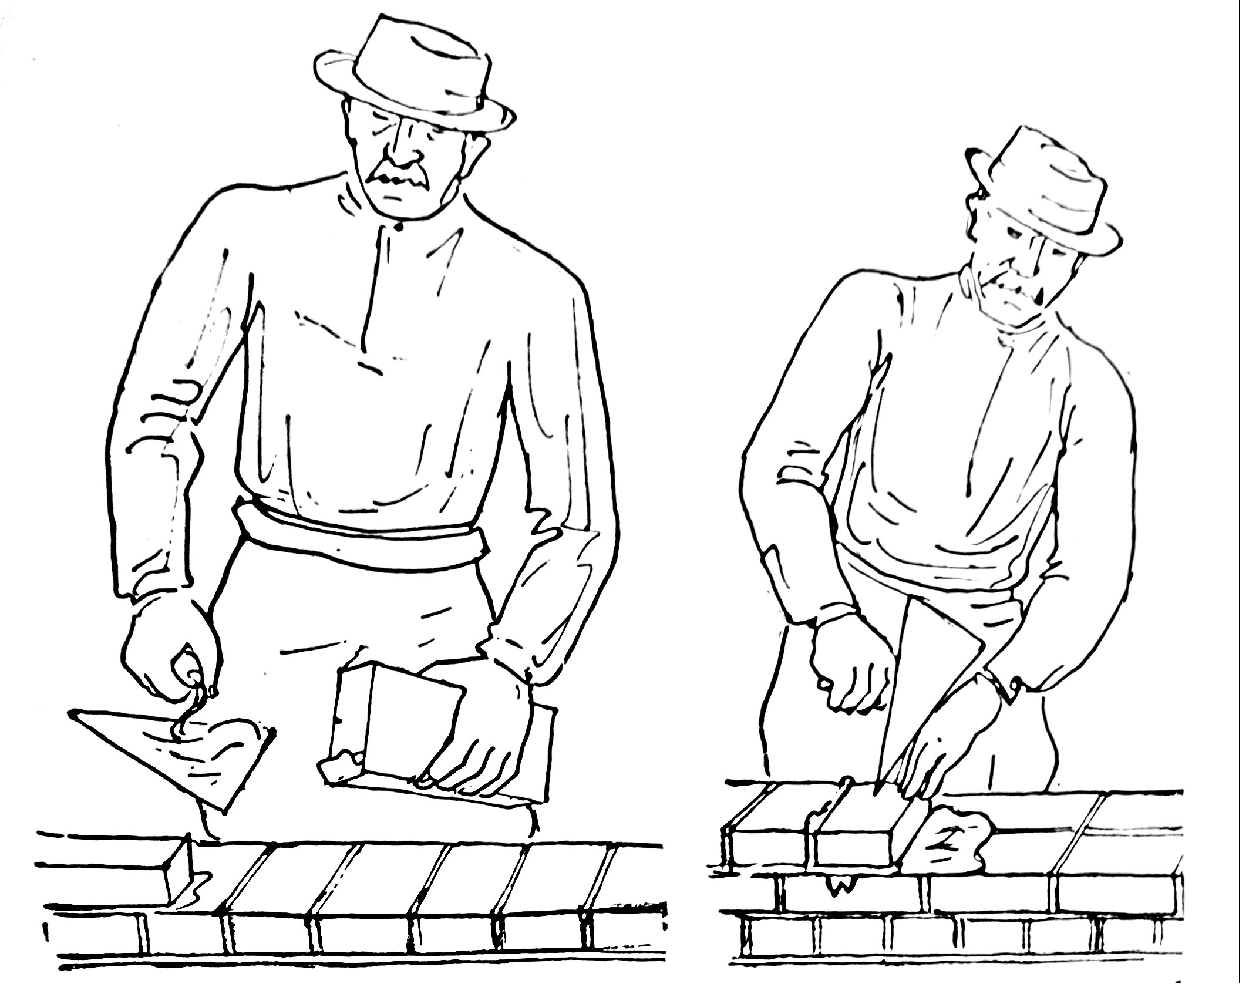
\includegraphics[width=0.45\linewidth ]{figure/Introduction/bricklayer2.pdf}
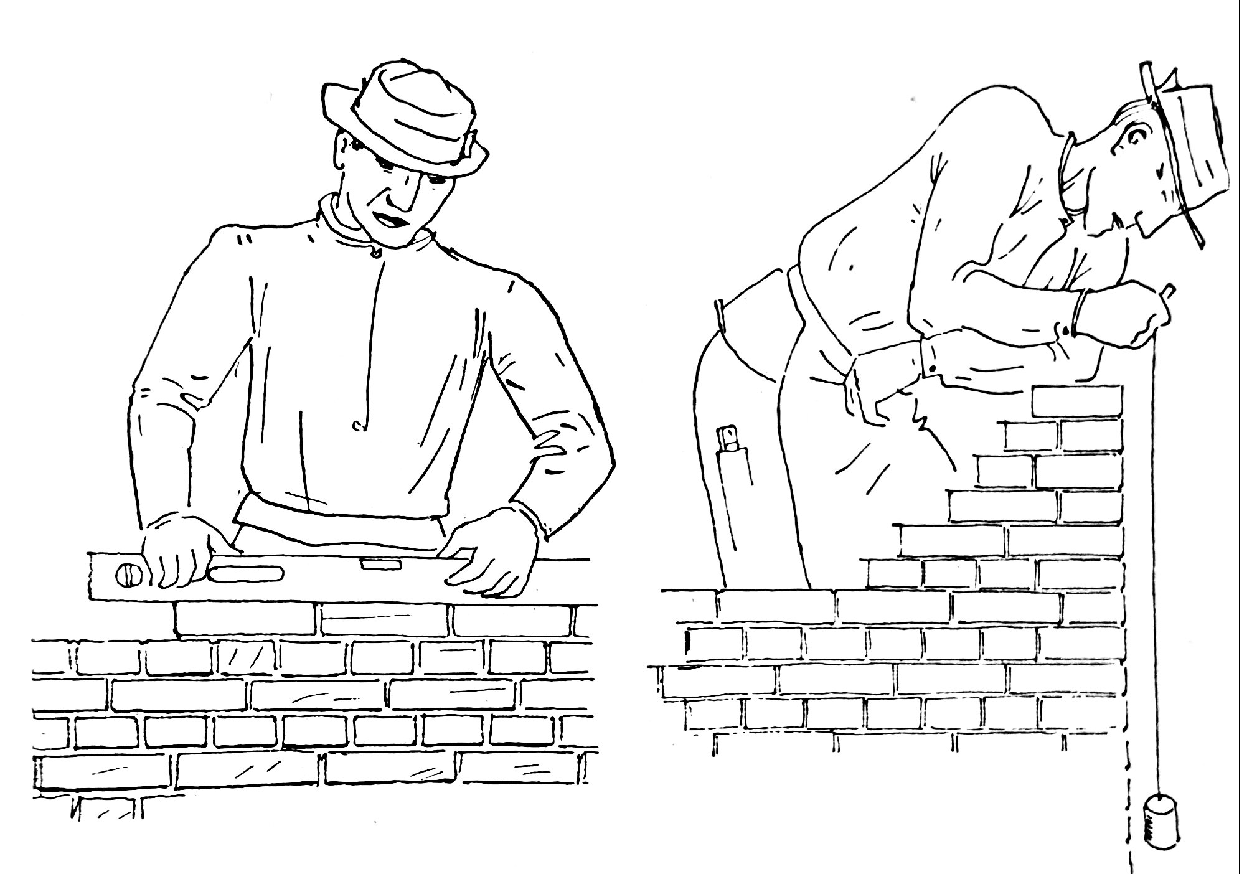
\includegraphics[width=0.45\linewidth ]{figure/Introduction/bricklayer1.pdf}
\caption{The length of the curve is the same regardless of coordinate system.\cite{ref:murning}}
\label{fig:murning2}
\end{figure}



There have not been many alternatives to this quite traditional way of bricklaying. Methods have been made to combine concrete elements with bricks or using brick laying robots. These techniques give some possibilities that might be hard to achieve using traditional methods. A big difference is that you often get a industrial feeling, meaning perfect results, and you loose the human touch.

\begin{figure}[H]
\centering
\includegraphics[width=0.8\linewidth ]{figure/Introduction/RobotBrick.jpg}
\caption{ETH Brick Robot}
\end{figure}



\subsection{Production and Realization}

An important part of design is the physical realization of the drawings. The vault is an interesting example since the structure usually is very weak until the keystone or brick finishes the geometrical shape. This problem has puzzled engineers and architects for a long time and the solution to this problem has been a bit different historically depending on which part of the world your at. One can say that there have been three different paths: \cite{ref:Dieste}

\begin{enumerate}
    \item The European
    \item The Middle Eastern
    \item The Catalan
\end{enumerate}


\begin{figure}[H]
\centering
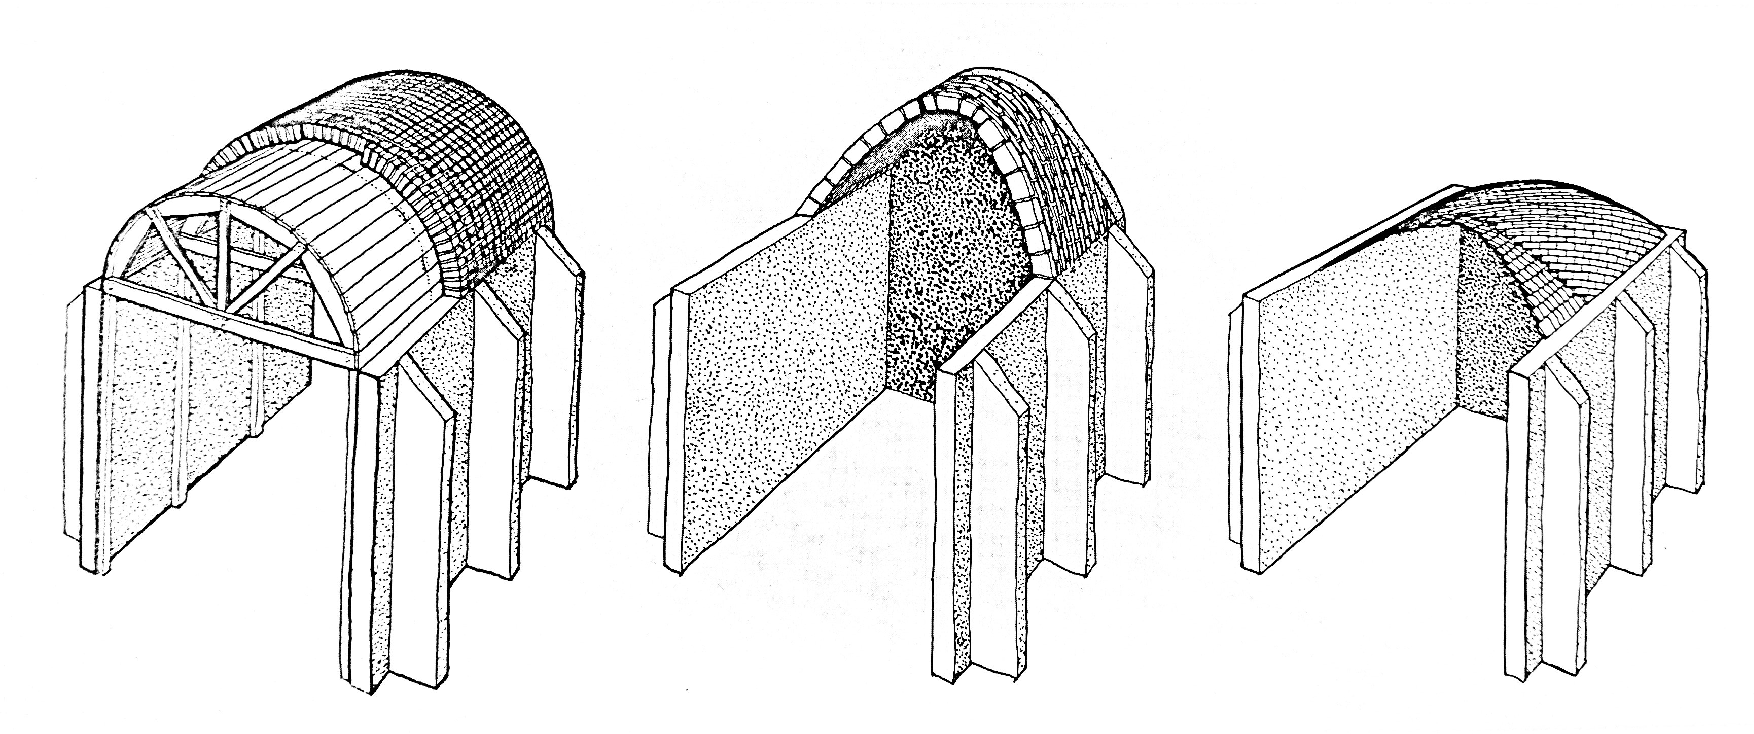
\includegraphics[width=0.9\linewidth ]{figure/Introduction/vaulting2.pdf}
\caption{The three main types vaulting, to left the European vault that is usually round and requires form work, the middle is the Middle Eastern Vault which tends to be parabolic shape and to the right the Catalan vault which are thinner and lighter and has multiple layers \cite{ref:Ochsendorf}}
\label{fig:vaults}
\end{figure}


The European path includes vaulting techniques from time eras such as Roman, Romanesque, Gothic and Renaissance. The common factor for them is that they usually are based on a circle, such as barrel vault, and they often require temporary centering or form work to stabilise the construction until the vault is finished. They are often relatively thick and they the bricks often follow the radial lines \cite{ref:Dieste}. Looking at the vaults and brick patterns and vaults in section \ref{sec:brickPatt} and \ref{sec:masonryShells} ,which are from a Swedish textbook, proves that the technique evolved with time, and to reduce the weight special bricks which are lighter than normal bricks \cite{ref:murning}. This can be seen in pictures where the form-work is only partial and the bricks are only kept in place by the mortar, which is is not possible with solid bricks. In figure \ref{fig:kryssvalv}a),  one can see the construction of a brick vault. Until the beginning of the 20th century it was required of a Swedish brick layers to by them self raise a vault with only a wooden template telling the curvature\cite{ref:murning}, as in figure \ref{fig:kryssvalv}b). This tells how dependent the end result was based on the intuition and experience of the brick layer. Unfortunately this knowledge is since long gone, or it is a talent of very few, these days.

\begin{figure}[H]
\centering
\includegraphics[width=1.0\linewidth ]{figure/Introduction/makingkryssvalv.pdf}
\caption{Until the beginning of the 20th century it was required of a Swedish brick layers to by them self raise a vault with only a wooden template telling the curvature\cite{ref:murning}}
\label{fig:kryssvalv}
\end{figure}

The Middle Eastern vaults, in comparison to the European tended to be parabolic in its shape. The technique of vaulting is a bit different since the courses were inclined towards a wall or stiff end and therefore get support. The more efficient shape and vaulting technique meant that form-work not necessarily needed\cite{ref:Dieste}, see figure \ref{fig:vaults}b)
The Catalan vaults, or Mediterranean tile vaulting, is rather different than its two relatives. While the others use bricks or stones these are much thinner and more related to tiles. This means that they can be made much thinner and they are often laminated into multiple layer. The lamination and the small thickness makes it light and strong\cite{ref:Dieste}. The Catalan vaults can also be much shallower than the other vaulting methods, which is a possibility due to its low weight. Oschendorf distinguish two key feautres compared to other types of vaulting, \textit{ Two key features distinguish tile vaulting from other types of vaulting from other types of masonry vaulting. First, thin tiles are laid flat to constitute the surface of the vault, joined along their thin edges, in contrast to vertical orientation of masonry units in traditional construction.Secondly, the first layer of tiles is joined with plaster, which sets so quickly that tiles are held in place almost instantaneously, and there is no need for support from below during construction.}\cite{ref:Ochsendorf}
\vspace{5mm}

It is shown that the primary reason for form-work historically has been to stabilize the structure during erection, rather than for the brick layer to understand the form or surface. For more complex surfaces double-curved structures the same of argument will not hold an more references are needed to understand the surface. In the complex vault, or shell, constructed and designed by the BRG at ETH campus is an example of such a case, see figure \ref{fig:ethvault}. For that project a quite extensive form-work was made by CNC cut cardboard plates.\cite{ref:Davis}
 

\begin{figure}[H]
\centering
\includegraphics[width=0.49\linewidth ]{figure/Introduction/VaultBlock2.jpg}
\includegraphics[width=0.49\linewidth ]{figure/Introduction/VaultBlock.jpg}
\caption{The length of the curve is the same regardless of coordinate system.}
\label{fig:ethvault}
\end{figure}


\subsection{Finding forms of equilibrium} \label{sec:findingform}

The term form-finding usually refers to the process of finding a shape that is in static equilibrium under a certain design load. This usually applies to shapes of shells or membranes where an efficient geometry is hard to conceive using analytical reasoning. Linkwitz expresses it as,
\textit{"As part of the conceptual design of structures, especially domes, shells and membrane structures, generating adequate structural shape is crucial to the load-bearing behaviour and aesthetic  expression of design.Their shapes cannot be freely chosen and conceived directly, due to the intrinsic interaction between form and forces. For such a problem one needs \textit{form finding}.}" \cite{ref:ShellOpt}

Typical structures that require form finding include:

\begin{itemize}
\item soap films within a given boundary.
\item prestressed, or hanging fabric membranes.
\item prestressed, or hanging cable nets.
\item structures generated by pressure.
\end{itemize}

Even though it is a design approach implies that the structure should find its position of rest the designer has measures of controlling and influence the outcome. One can speak of different parameters that the designer controls and impose.\cite{ref:ShellOpt} 

\begin{itemize}
\item \textit{Boundary Conditions}, which implies the supports and external loads.
\item \textit{Topology and Geometry}, what is the initial geometry and how are all members connected.This decides how and where the forces are allowed to move.
\item \textit{Internal forces}, this controls how the forces are distributed and transferred internally. 
\end{itemize}

There are different methods that applies to form-finding. In recent years with more powerful computers some numerical methods not possible has previously has been available. The art of form finding though goes back in history, and the simplest method can be performed with a pencil and ruler. 

\subsubsection{Graphical Methods}

The most basic type, but not less powerful, of form finding is graphical methods. A type of these is called \textit{graphic static} or \textit{force polygon method}. This method can be used to seek a form of equilibrium or analysing already designed structural members such as trusses. The method originates from the work of \textit{Karl Culmann} published in \textit{Die graphische statik} in 1866.This method have had much influence for modern structural design in the late 19th century and early 20th century and was used by modern structural pioneers such as \textit{Rafael Guastavino,Antoni Gaudi,Felix Candela} and \textit{Robert Maillart}. 

\begin{figure}[H]
\centering
\includegraphics[width=0.6\linewidth ]{figure/Introduction/GraphStat4.JPG}
\caption{Compression-only Form finding through Finite Subdivision of the
Force Polygon\cite{ref:Form} }
\end{figure}

The main idea is to use work in this force polygons which are represented in what is called a reciprocal force diagram. These polygons should always be closed to ensure that the forces are in equilibrium. In the example below, from the book Form and Forces, it illustrates a hanging cable where the internal forces and global forces are constructed as triangles, and since they are closed polygons the structure is in equilibrium. The powerful aspect of graphic statics is the illustrative way of expressing the force connections and how the design relates the force patterns.   


\begin{figure}[H]
\centering
\includegraphics[width=0.6\linewidth ]{figure/Introduction/GraphStat2.JPG}
\includegraphics[width=0.35\linewidth ]{figure/Introduction/GraphStat3.JPG}
\caption{Compression-only Form finding through Finite Subdivision of the
Force Polygon \cite{ref:Form} }
\end{figure}


\subsubsection{Analytical Methods}

For some cases is possible to analytically derive the shapes of funicular arches and shells, i.e only axial forces. It is not very common since it easily gets very complicated applying it to complex demands on a structure, both architectural and structural. For simple arches and shell it is though possible by assuming for instance constant loading,internal forces or stresses.  Chris Williams describes in the book \textit{Shell Structures for Architecture} how to attain the mathematical expressions for both arches and shells, with varying constraints.
You might also read \textit{ Tensile Structures Volume 2,  Cable nets} by Frei Otto for a descriptive way to analytically describe single cables and cable nets analytically. 

\begin{figure}[H]
\centering
\includegraphics[width=0.6\linewidth ]{figure/Introduction/constantShell.pdf}
\caption{Constant stress shells of derived analytically by Chris Willams. }
\end{figure}


\subsubsection{Physical methods}

Using physical models to understand and communicate design has been a vital part in proceeding in the field of structural engineering. Many have seen the the hanging cable models of \textit{Gaudi} but the modern pioneers in this field was structural engineers and architects such as \textit{Frei Otto} and \textit{Heinz Isler}. During the 20th century both of them elaborated with physical models to understand the shapes and design of light weight structures. Otto is most known for his works with membrane structures and soap film models, while Isler worked more with compression shells.\cite{ref:Isler}
\begin{figure}[H]
\centering
\includegraphics[width=0.6\linewidth ]{figure/Theory/Soap.jpg}
\caption{The tangent differs depending of which direction you refer to. }
\end{figure}

Today this is mostly a done by architects communicating their design and understand geometrical affects on spaces. Even though physical models and testing is one of most optimal ways to validate theory it is no longer part of the structural engineering culture to do so. The need for physical models can be for various reasons.\textit{ 
"Designers of structures have used small-scale models when it is beneficial to do so, especially in order to raise the engineers confidence in the design being proposed. This may have been for many reasons. For example:"}  \cite{ref:ShellOpt}

\begin{itemize}
\item The available calculation methods were to complex or time-consuming
\item it would be too costly to build a full-size prototype
\item it was believed that normal structural analysis methods would not adequately model the structure.
\item the geometry of the structure could not be defined using a mathematical equation
\item there were no other means available
\end{itemize}





\subsubsection{Numerical Methods} \label{numerical Methods}

The numerical methods for form-finding are usually spoke of them as quite different, but they all share the same basic ideas. In the book Shell.. they formulate a recipe for a numerical form-finding method:\\

\begin{enumerate}
    \item \textit{Discretization of geometry}. This means that the initial geometry or form needs to be broken down into elements such as lines or surface elements.
    \item \textit{Connectivity of internal and external forces}, it is necessary to have a clear topology of how the members are connected and how the external loading and boundary conditions apply.
    \item \textit{Equilibrium conditions and equations}. The equilibrium conditions defines how the internal and external forces and boundary relate to each other. 
    \item \textit{A solver}, a method for how the equilibrium equations can be solved.
\end{enumerate}
\vspace{5mm}

This template is of course a bit rough and there is a big diversity of solvers, it can be linear or non-linear problems and it can be a static or dynamic equilibrium conditions for instance. To give a bit of structure to this diversity Block and Veenendaal describes different \textit{form-finding families}.\\ 


\begin{enumerate}
\item \textit{Stiffness Matrix Methods}, these are based on using standard elastic and geometric matrices. These have a strong connection to traditional structural analysis and \textit{Finitie Element Method(FEM)}.
\item \textit{Geometric Stiffness Methods}, these are material independent where the equilibrium is achieved only with a geometrical stiffness. The most common and influential of these is the \textit{Force Density Method(FMD)}, where the equilibrium equations are based on the ratio of force to length. Extensions have been done and different methods have been emerged such as the \textit{Thrust Network Analysis(TNA)}.
\item \textit{Dynamic Equilibrium Methods}, these methods have a dynamic based equilibrium condition, i.e the second Law of Newton $\sum F = ma$ which is different compared to statics where the sum of forces always are equal to zero. Examples of these methods are \textit{Dynamic Relaxation(DR)} and \textit{Particle-Spring(PS)} systems. You can read further about DR in section \ref{DR}. The figure \ref{fig:DR} can give an idea of how a DR or PS can behave for a quadratic mesh fixed in the corners. 
\end{enumerate}

\subsection{Computational Design in Architecture}

Design in architecture often refers to creative design process where you explore different options related to specific task or conditions. The term "Thinking outside the box" is somewhat positive in the modern architecture in aspiration of new architecture. Computers on the other hand are bound to think inside the box based on logic rules.Though they are much more efficient in handling data and calculations then we humans do. Computational design can be seen as the merge of these two design concepts, thinking outside the box inside the box. The combination makes it possible to solve difficult problems that demands huge computational power or generate designs hard to imagine beforehand. 

Offices  that was early in defining units specialized in computational design and complex problem are \textit{Foster and Partners},\textit{ Arup} and \textit{Buro Happold}. Today there are more offices and academic institutes that specializes in this area.

\begin{figure}[H]
\centering
\includegraphics[width=0.9\linewidth ]{figure/Introduction/ICD.jpg}
\caption{Research pavilion 2011 designed by the Institute of Computational Design (ICD) }
\end{figure}

\subsubsection{Parametric Design}
Parametric Design is relatively new concept in Architecture that has been developed during the late 20th century and beginning of 21th century, and the development continues. 

"In parametric design it is the parameters of a particular design that are declared and not its shape. By assigning different values to the parameters, different objects or configurations can be created." Smart geometry
It is a way of seeing the design process as a rule-based system, which can be refereed as \textit{algorithmic thinking}."Algorithmic thinking allows designers  to rationalize, control, iterate, analyze and search for solutions in a defined solution space." Parametric Design for Architecture.
Examples of environments using a parametric concept is \textit{Grasshopper3d}, \textit{Dynamo} and 
\textit{Generative Components}.

\subsubsection{Design Scheme} \label{dScheme}

\begin{figure}[H]
\centering
\includegraphics[width=1.0\linewidth ]{figure/Introduction/DesignScheme.pdf}
\caption{The tangent differs depending of which direction you refer to. }
\end{figure}

\subsection{Pre-study of different thesis questions}
In this section I will describe a two week long workshop where the purpose was to investigate different tracks in the context explained in the previous sections. 

\subsubsection{Comparison of different form finding methods} \label{CompMethods}
There are a range of different numerical methods for exploring form which was discussed briefly in section \ref{numerical Methods}. They are often mentioned as different but maybe it is also true to say they are very equal in the sense that all of them seeks equilibrium. There is a difference in the sense that they demand different parameters, some give a lot of options and some can be very simple in their most basic implementation, they can be more or less computational heavy and maybe more or less suiting for the kind of situation. 
Reading about the different methods, in Architecture..., a basic implantation was made for \textit{Force Density}, a simplified version of \textit{TNA} and \textit{Dynamic Relaxation}. This was done in Grasshopper components. 


\begin{figure}[H]
\centering
\includegraphics[width=0.9\linewidth ]{figure/Introduction/PreStudyComp.png}
\caption{The tangent differs depending of which direction you refer to. }
\end{figure}

Possible research questions in this field:
\begin{itemize}
\item \textit{Computational power} - As designers and engineers we like to be able to get real time response. If the algorithm demands a lot of computational power it can be a limiting factor in regards of extending the functionality. 
\item \textit{Extendability} - Is it possible to be able to implement more functionality and more advanced or complex models.
\item \textit{Designer friendly} - Sometimes we are given to many, or to few parameters, to actually control the output. Who is the designer? And what does he or she need to know. 
\end{itemize}

\subsubsection{Parametric design tools}
There is a big difference in doing manual editing such as typical 3d-modelling and doing a fully parametrized design where need communicate with conditional statements and different sliders. There are big advantages in having a intelligent design, it can though also be limiting when you want to tweak your design in a way you can´t describe in scripts. A possibility would be to combine the two approaches to give some freedom and some intelligence. A parametric definition you can change and alter and a freedom to also do some manual tweaking.\\

A simple example was made using the on of the methods developed in the previous section \ref{CompMethods} . Inspired by a picture of free-form masonry arch where you can design the arch and see if it is possible to find an equilibrium solution that fits the form.

\begin{figure}[H]
\centering
\includegraphics[width=0.6\linewidth ]{figure/Introduction/PreStudyDes.png}
\caption{The tangent differs depending of which direction you refer to. }
\end{figure}


\begin{figure}[H]
\centering
\includegraphics[width=0.9\linewidth ]{figure/Introduction/PreStudyDes3.png}
\caption{The tangent differs depending of which direction you refer to. }
\end{figure}

Possible extension to this field might be to develop algorithms and parametric definitions that give more freedom for designer and also give feedback if it is suitable or not, or searches for the closest possible to solution. An example can be related to the design of domes where it is a form that the designer has found appealing though history, but it is not really optimal since the form itself creates tension. Though we can find a solution that fits inside by adjusting boundaries and weights.

\subsubsection{Visualization and structural understanding }

The software \textit{RhinoVault} is based on the methodology of TNA, and is made for \textit{Rhinoceros3d}. It provides some really nice features such as the reciprocal force diagrams that are visualized and possible to change and adapt to the structure. It gives another kind of understanding of how the forces are connected than typical gradient based force diagrams, just showing high and low stresses. It powerful feature that can be applied in a parametric environment where you can connect all the powerful features of a parametric design environment. A proposal of using dynamic relaxation create a reciprocal force diagram was made by Daniel Piker. Connecting the form-finding methods developed in \ref{CompMethods} you can get some real nice projected force diagrams. In this way he states though that it is only a one way connection and so you cannot two-way connection as in RhinoVault. This implies only applying the same force densities or stiffness to the members which is rather limiting.

\begin{figure}[H]
\centering
\includegraphics[width=0.9\linewidth ]{figure/Introduction/PreStudyAna.png}
\caption{The tangent differs depending of which direction you refer to. }
\end{figure}

A possible research question would be to develop a software for parametric environments that gives the same functionality as in TNA to understand and interact with the reciprocal force diagrams.

\subsubsection{Physical testing of theoretical methods}
\begin{figure}[H]
\centering
\includegraphics[width=0.9\linewidth ]{figure/Introduction/PreStudyFab.png}
\caption{The tangent differs depending of which direction you refer to. }
\end{figure}


\section{Purpose} 
The  purpose of this thesis is to investigate the possibility of using the concepts of differential geometry to generate the patterns for bricklaying on compressive shell forms. The report will integrate the fields theory of differential geometry, theory of shells, theory of masonry structures and computational methods. The theoretical framework will therefore be divided in four parts:\\
\begin{enumerate}
    \item \textit{Theory structural masonry} - This will be based on a plastic design approach used for assessment and understanding of complex historical masonry structures such as cathedrals. The theory differs from traditional structural engineering practice due to the nature of the masonry composition where stresses in structure cannot be read in the same way.   
    \item \textit{Differential geometry} - This section will explore the basics of differential geometry which includes the elementary theory related to curves and surfaces. This is a necessity for understanding the theory of free-form shells. The part will also include parts that are not directly related but can be confusing if not explained, for instances there are different types of curvature for surfaces and curves and it is necessary not to mix them up.
    \item \textit{Theory of free-form membrane shells} - This section will describe the theory of free-form shells in a approach understandable for the structural engineer. This complex theory is usually used by mechanical engineers and no attempts has been done to explain in the concepts for the structural engineer.
    \item \textit{Computational methods} - This section will explain how computational methods can be used to find solutions when the analytical solutions based on the theory above can´t or is very hard to achieve.
\end{enumerate}


\section{Limitations} \label{Section_ref}

This report will only concern brick structures, meaning module blocks with the same dimensions, and not other types of masonry structures such as stone or concrete. The structural theory though applies to all masonry structures. The report will concern compressive brick shell structures and not conventional brick structures. Compression structures meaning in this case structures where the form ensures equilibrium in compressive axial forces and where reinforcement is not necessary in theory. The forms generated are of conceptual nature meaning that no detailed calculations or instability checks are made, such as buckling. \\ 

The implementations will be programmed in a parametric development environment,but no effort will be made to develop and evaluate different parametric design processes. The code will be implemented using the object-oriented language C\#. The methods are though general and should be possible to implement using most languages. 

\section{Method} \label{Sec:method}

Below is a description a process and its  different stages that will be the guide of the work of this thesis.

\begin{enumerate}

\item \textit{A literature review} will be executed which investigates historical and new knowledge and research in the fields related to masonry structures: tessellation and geometry,form and function, production  and computational methods. The literature review will be the foundation that with a contextual view of different areas crystallizes into a research question.
\item \textit{ An in depth theoretical study and gathering} will be done in fields coinciding with relevance for the research question developed in previous stage and the limitations made.  
\item From the theoretical foundation \textit{a process or method} will be made as a possible way of achieve or answer the research question made.
\item The method will be implemented and the results will be presented. The results will be the foundation of a \textit{discussion} that reviews the method and the validity of the results.
\item A list of possible areas of improvements and possible future research will be presented.
\end{enumerate}
